\documentclass{article}

% Formatting
\DeclareUnicodeCharacter{2060}{\nolinebreak} % Prevent unicode (U+2060) error on local complile
\frenchspacing % No double spacing between sentences
\hbadness=1000000 % Turn off \hbox badness warnings
\linespread{1.2} % Set linespace


% Packages
\usepackage[a4paper, left=1.5cm, right=1.5cm, top=1.5cm, bottom=1.5cm]{geometry}
\usepackage{array} % For allowing new column types in tables
\usepackage{authblk} % For author formatting
\usepackage{caption} % For figure and table captions
\usepackage{cclicenses} % For creative commons license
\usepackage{float} % To force figure location after text
\usepackage{graphicx} % Adds more functionality to graphics for inclusion of figures
\usepackage{lscape} % For landscape pages
\usepackage{lineno} % Allows use of \linenumbers to add line numbers 
\usepackage{lmodern} % A scalable font - avoids erros due to non-sclabale fonts
\usepackage{longtable,booktabs}  % For tables
\usepackage{markdown} % allow use of markdown syntax
\usepackage{microtype} % 'Improved' typesetting
\usepackage[nottoc,numbib]{tocbibind} % Add references to table of contents
\usepackage{parskip} % Adds white space between paragraphs
\usepackage{pdflscape} % To create landscape pages that show as landscape in PDF viewer
\usepackage{ragged2e} % Better right ragged edges (allows hyphenation)
\usepackage{subcaption} % Allows use of subfigures and subtables
\usepackage{subfig} % Allows use of subfigures and subtables
\usepackage[super]{natbib} % Citations using superscript
\usepackage{titlesec} % For title spacing
\usepackage[toc,page]{appendix}
\usepackage{url} % Tidy web links
\usepackage[utf8]{inputenc}
\usepackage{verbatim}
\usepackage{xcolor} % For coloured text
\usepackage{xurl} % For url but with more flexible linebreaking


% Choose your own colour
\usepackage{color}
\newcommand{\mjanote}[2][\textcolor{red}{\dagger}]{\textcolor{red}{$#1$}\marginpar{\color{red}\raggedright\tiny$#1$ #2}}
\newcommand{\mjaFIXME}[1]{\textcolor{red}{[\textbf{FIXME} \textsl{#1}]}}
\newcommand{\kpnote}[2][\textcolor{magenta}{\dagger}]{\textcolor{magenta}{$#1$}\marginpar{\color{magenta}\raggedright\tiny$#1$ #2}}
\newcommand{\kpFIXME}[1]{\textcolor{magenta}{[\textbf{FIXME} \textsl{#1}]}}


% Info on wordcounts:
% https://www.overleaf.com/learn/how-to/Is_there_a_way_to_run_a_word_count_that_doesn%27t_include_LaTeX_commands%3F

% To include refs in word count:
%TC:incbib


\newcommand{\detailtexcount}[1]{%
  \immediate\write18{texcount -merge -sum -q #1.tex output.bbl > #1.wcdetail }%
  \verbatiminput{#1.wcdetail}%
}

\newcommand{\quickwordcount}[1]{%
  \immediate\write18{texcount -1 -sum -merge -q #1.tex output.bbl > #1-words.sum }%
  \input{#1-words.sum} words%
}

\newcommand{\quickcharcount}[1]{%
  \immediate\write18{texcount -1 -sum -merge -char -q #1.tex output.bbl > #1-chars.sum }%
  \input{#1-chars.sum} characters (not including spaces)%
}

% Count tables in wordcount

%TC:group table 0 1
%TC:group tabular 1 1

\begin{document}


% Ignore title and abstract in word count
%TC:ignore
\title{Identifying levers for improving thrombolysis use and outcomes – combining clinical pathway simulation and machine learning applied to the UK stroke registry}


\renewcommand{\thefootnote}{\fnsymbol{footnote}}
\author[1,2]{Kerry Pearn}
\author[*1,2]{Michael Allen}
\author[1,2]{Anna Laws}
\author[3]{Peter McMeekin}
\author[1,2]{Martin James}

% Check affiliations - update RDE Name
\affil[1]{\footnotesize University of Exeter Medical School}
\affil[2]{\footnotesize NIHR South West Peninsula Applied Research Collaboration (ARC)}
\affil[3]{\footnotesize Northumbria University}
\affil[*]{\footnotesize Corresponding author: m.allen@exeter.ac.uk}
\maketitle
%TC:endignore
\section*{Abstract}

Background: Stroke is a common cause of adult disability. Expert opinion is that about 20\% of patients should receive thrombolysis to break up a clot causing the stroke. Currently, 11–12\% of patients in England and Wales receive this treatment, ranging between 2\% and 24\% between hospitals.

Objectives: By combining clinical pathway simulation and machine learning of thrombolysis decision-making and outcomes, we sought to better understand the source of variation in thrombolysis use and the effect on outcomes.

Methods: Monte-Carlo simulation was used to model the flow of patients through the emergency stroke pathway at each hospital, taking into account both average speeds and variation. XGBoost machine learning models were used to learn which patients would receive thrombolysis at each stroke team, and learn and predict outcomes with and without thrombolysis. The models were used to predict the effect of alternative improvement strategies.

Results: Combining potential changes (improving arrival-to-thrombolysis times to 30 mins, reducing ambulance call-to-hospital-arrival times by 15 minutes, having all teams attain the current upper-quartile performance in determining stroke onset time (79.6\%), and applying decision making similar to high thrombolysing units) would be expected to increase thrombolysis use in patients arriving by ambulance from 13\% to 20\% and double the clinical benefit (additional patients discharged mRS 0-1) from thrombolysis. The largest single factor is differences in clinical decision-making, especially around mild stroke (which make up half of all stroke admissions). Using our outcome machine learning we found that high thrombolysing units are predicted to be generating more net benefit (including better avoidance of mortality and severe disability) than low thrombolylsing units. A health economics model, using the output from the outcome prediction model, estimated that thrombolysis produces an additional 0.26 QALY for each person treated.

Conclusions: There is significant inter-hospital variation in use of thrombolysis that is caused by hospital processes and differences in decision-making. Improving processes and adopting the decision making of higher-thrombolysing units would be expected to improve both thrombolysis use and outcomes. Pathway analysis and machine learning should allow stroke teams to better understand, and improve, their own pathways.

\section*{Plain Language Summary}

\textbf{What is the problem?} Use of clot-busting treatment (`\textit{thrombolysis}') in stroke varies a great deal between hospitals.

\textbf{What did we know?} We knew that the largest cause of this variation was in how doctors decide which patients are suitable for thrombolysis. We knew other significant causes of variation were how fast hospitals can decide who to give thrombolysis to (which requires a specialist head scan). Hospitals also vary in how many patients they work out when the patient had their stroke.

\textbf{What did we not know?} We did not know how addressing all these causes of variation in thrombolysis use and speed would affect the number of people who receive thrombolysis and, most importantly, how patient outcomes would change.

\textbf{What did we do?} We used machine learning to find patterns in which patients each hospital gives thrombolysis to, and how that thrombolysis affects patient outcome. We used clinical pathway simulation to simulate, in a computer, many patients moving through each hospitals emergency stroke pathway. We use this simulation model to test changes to the pathway (such as making it faster), and see what the likely effect of thrombolysis use and patient outcomes would be.

\textbf{What did we find out?} We found that use of thrombolysis could be increased from 13 patients in 100 being given it, to 20 patients in 100 being given. But each hospital should have its own target which takes into account their local population. We found that overall, the benefit from thrombolysis could be doubled - with more patients receiving it and with patients receiving it earlier which gives all those patients a better chance of being discharged from hospital able to live independently.
\section{Introduction}

% Include
% 1) What is the problem?
% 2) What do we know about low and varying use of thrombolysis
% 3) What do we not know
% 4) How are we addressing what we don't know

% 1) What is the problem?

Stroke remains one of the top three global causes of death and disability \cite{feigin_global_2021}. Despite reductions in age-standardised rates of stroke, ageing populations are driving an increase in the absolute number of strokes \cite{feigin_global_2021}. Across Europe, in 2017, stroke was found to cost healthcare systems \texteuro 27 billion, or 1.7\% of health expenditure \cite{luengo-fernandez_economic_2020}. Thrombolysis with recombinant tissue plasminogen activator, can significantly reduce disability after ischaemic stroke, so long as it is given in the first few hours after stroke onset \cite{emberson_effect_2014}. Despite thrombolysis being of proven benefit in ischaemic stroke, use of thrombolysis varies significantly both between and within European countries \cite{aguiar_de_sousa_access_2019}. In England and Wales the national stroke audit reported that in 2021/22, 20 years on from the original European Medicines Agency licencing of alteplase for acute ischaemic stroke, thrombolysis rates for emergency stroke admissions varied from just 1\% to 28\% between hospitals \cite{sentinel_national_stroke_audit_programme_ssnap_2022}, with a median rate of 10.4\% and an inter-quartile range of 8\%-13\%, against a 2019 NHS England long term plan that 20\% of patients of emergency stroke admissions should be receiving thrombolysis \cite{nhs_long_term_plan_2019}. The NHS plan for improving stroke care also sets a target that patients should receive thrombolysis within 60 minutes of arrival, but ideally within 20 minutes. Whilst this speed of thrombolysis, called door-to-needle time, provides an ambitious target, it has been shown to be achievable as Helsinki University Central Hospital has reported a median door-to-needle time of 20 minutes, with 94\% of patients treated within 60 minutes \cite{meretoja_reducing_2012}.

% 2) What do we know about low and varying use of thrombolysis

Studies have shown that reasons for low and varying thrombolysis rates are multi-factorial. Reasons include late presentation \cite{aguiar_de_sousa_access_2019}, lack of expertise \cite{aguiar_de_sousa_access_2019} or lack of clear protocols or training \cite{carter-jones_stroke_2011}, delayed access to specialists \cite{kamal_delays_2017}, and poor triage by ambulance or emergency department staff \cite{carter-jones_stroke_2011}. For many factors, the establishment of primary stroke centres has been suggested to improve the emergency care of patients with stroke and reduce barriers to thrombolysis \cite{carter-jones_stroke_2011}, with a centralised model of primary stroke centres leading to increased likelihood of thrombolysis \cite{lahr_proportion_2012, morris_impact_2014, hunter_impact_2013}. 

In addition to organisational factors, clinicians can have varying attitudes to which patients are suitable candidates for thrombolysis. In a discrete choice experiment \cite{de_brun_factors_2018}, 138 clinicians considered hypothetical patient vignettes, and responded as to whether they would give the patients thrombolysis. The authors concluded that there was considerable heterogeneity among respondents in their thrombolysis decision-making. Areas of difference were around whether to give thrombolysis to mild strokes, to older patients beyond 3 hours from stroke onset, and when there was pre-existing disability.

Based on national audit data from three years of emergency stroke admissions, we have previously built models of the emergency stroke pathway using clinical pathway simulation to examine the potential scale of the effect of changing two aspects of the stroke pathway performance (1. the in-hospital process speeds, and 2. the proportion of patients with a determined stroke onset time), and using machine learning to examine the effect of replicating clinical decision-making around thrombolysis from higher thrombolysing hospitals to lower thrombolysing hospitals \cite{allen_using_2022, allen_use_2022}. The machine learning model learned whether any particular patient would receive thrombolysis in any particular emergency stroke centre. Using these models we found that it would be credible to target an increase in average thrombolysis in England and Wales, from 11\% to 18\%, but that each hospital should have its own target, reflecting differences in local populations. We found that the largest increase in thrombolysis use would come from replicating thrombolysis decision-making practice from higher to lower thrombolysing hospitals. Two other important factors influencing thrombolysis rates were determination of stroke onset time in some hospitals, and improving the speed of the in-hospital thrombolysis pathway.

There is also a question in the literature of the benefit of thrombolysis in mild stroke. Patients with mild stroke (NIH stroke scale $<5$) make up half of emergency stroke admissions \cite{allen_using_2022}, but they only were present in the clinical trials at a bit lower than 10\% of the trial population \cite{emberson_effect_2014}. Though the clinical trial meta-analysis supported use of thrombolysis in mild stroke \cite{emberson_effect_2014}, other studies \cite{romano_predictors_2021, coutts_tenecteplase_2024} have suggested that use of thrombolysis in mild stroke may not be beneficial, or may cause harm. 

% 3) What do we not know

In our previous work we established that we could predict the use of thrombolysis in patients arriving within 4 hours of known stroke onset with 84.3\% accuracy \cite{allen_use_2022}. We could then ask the question "What if this patient attended another hospital - would they likely be given thrombolysis?" In that work, when we altered selection of patients for thrombolysis, we were only predicting thrombolysis choice; we were not examining outcomes after stroke with and without thrombolysis, which left open the question of whether stroke teams with higher thrombolysis use were likely to be achieving better outcomes. In this paper we extend the pathway model to examine outcomes after applying the predicted decision-making from higher thrombolysing hospitals, including a health economics analysis. As there is a question of use of thrombolysis in mild stroke, we also sought to better understand how thrombolysis use in that group of patients may be affecting outcome.
\section{Methods}

\subsection{Overview}

\begin{figure}
    \centering
    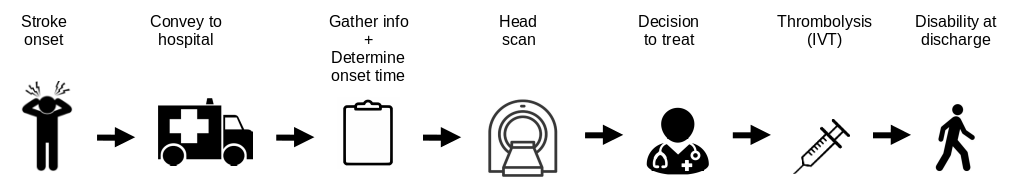
\includegraphics[width=1.0\linewidth]{images/flow}
    \caption{An overview of the process steps included in the modelling.}
    \label{fig:flow}
\end{figure}

Figure \ref{fig:flow} shows an overview of the process steps included in the modelling. Process flow was modelled by sampling from distributions of historic flow for each stroke team. Decision-making (choice of thrombolysis) was modelled with machine learning, learning which patients would likely be given thrombolysis at each stroke team. Outcomes were predicted using either mathematical models based on clinical trials (for the full pathway model), or clinical outcome machine learning models (for the more detailed analysis of differences in thrombolysis decision-making between teams).

\subsection{Data}

Data was used for all emergency stroke admissions to England and Wales for the 5 years 2017-2021, extracted from the national stroke registry for England, Wales and Northern Ireland, the Sentinel Stroke National Audit Programme (SSNAP). The registry contains all consecutive patients admitted to 100\% of acutely-admitting hospitals with a case ascertainment of over 90\% when compared to administrative data (Hospital Episode Statistics). Data was retrieved for teams with at least 250 admissions over the 5 years. The total number of patients was 302,715, of whom 114,625 (38\%) arrived within 4 hours of known stroke onset. Of those arriving within 4 hours of known stroke onset 103,244 (90\%) arrived by ambulance.

The following data fields from SSNAP were used in the modelling:

\begin{itemize}

    \item \textit{Stroke team}: Stroke team attended (hospital identifier).

    \item \textit{Age}: As midpoint of 5 year age bands.

    \item \textit{Sex}: Sex of patient (male/female)

    \item \textit{Diagnosis of atrial fibrillation}: Did the patient have a diagnosis of atrial fibrillation, either made prior to admission, or during admission?

    \item \textit{Use of anticoagulants}: Use of prior anticoagulant for atrial fibrillation.

    \item \textit{Onset known}: Whether onset was known, and if known whether it was considered to be known precisely or was a best estimate.

    \item \textit{Onset during sleep}: Did stroke occur in sleep? (1 = Yes, 0 = No).

    \item \textit{Onset-to-arrival time}: Time from onset of stroke to arrival at hospital (minutes), when known.

    \item \textit{Prior disability level}: Estimated modified Rankin Scale, mRS, prior to stroke.

    \item \textit{Stroke type}: Infarction/haemorrhage.

    \item \textit{Stroke severity}: National Institutes of Health Stroke Scale (NIHSS) score on arrival.

    \item \textit{Arrival-to-scan time}: Time from arrival at hospital to scan (minutes), when known.

    \item \textit{Scan-to-thrombolysis time}: Time from arrival at hospital to scan to treatment with thrombolysis  (minutes), when given.

    \item \textit{Disability on discharge}: mRS (0-6) on discharge, includes death (mRS 6) during admission.
    
\end{itemize}


\subsection{Thrombolysis decision model}

The thrombolysis decision model has been described in more detail previously \cite{pearn_what_2023}. Feature selection was used to identify 10 key features that were most predictive of whether thrombolysis was used in any given stroke team. The model uses XGBoost \cite{chen_xgboost_2016} for predictions, and SHAP \cite{lundberg_unified_2017} for local (patient-level) and global (model/population-level) explainability. SHAP values show the contribution of each feature value to the final model predictions.

The thrombolysis decision model was applied only to patients arriving within 4 hours of known stroke onset (stroke onset was known precisely or was a best estimate). The 10 features used for predicting thrombolysis use were: Stroke team; Age; Precisely known onset time; Onset during sleep; Onset-to-arrival time; Arrival-to-scan time; Stroke type; Stroke severity; Prior disability level; Use of anticoagulants.

Code, with demonstration, is available \cite{allen_samuel_code_2024}.

\subsubsection{Prototype patients}

To help compare decision-making and outcomes across stroke teams we exemplified differences using \textit{prototype patients}. These prototype patients captured a range of features known to affect decisions to treat, and to affect outcomes, and included an \textit{ideal} candidate for thrombolysis. The prototype patients used were:

\begin{enumerate}
    \item \textit{Ideal}: Onset-to-arrival = 90 minutes; arrival-to-scan = 15 minutes; onset-to-thrombolysis = 120 minutes; stroke severity (NIHSS) = 15; pre-stroke disability (mRS) = 0; age = 72.5; precisely known onset; onset not during sleep; stroke type = infarction; patient has no atrial fibrillation and is not receiving anticoagulants for atrial fibrillation.

    \item \textit{Late arrival}: As \textit{ideal} but onset-to-arrival = 225 minutes and onset-to-thrombolysis (when given) = 255 minutes.

    \item \textit{Mild}: As \textit{ideal} but stroke severity = 3.

    \item \textit{Prior disability}: As \textit{ideal} but pre-stroke disability = 3

    \item \textit{Imprecise}: As \textit{ideal} but stroke onset time estimated.

    \item \textit{Age}: As \textit{ideal} but age = 87.5.

    \item Combinations of the above.
\end{enumerate}

\subsubsection{Benchmark stroke teams and benchmark decisions}

SHAP isolates the contributes of features to model predictions. As one feature is the stroke team, the stroke team SHAP shows the influence of attending that stroke team on the likelihood of a patient receiving thrombolysis. Averaging stroke team SHAP values for all patients attending a given hospital provided a measure of the overall willingness of that stroke team to use thrombolysis (or how much that stroke team affected the odds of a patient receiving thrombolysis in the model). We took the stroke teams with the 25 highest stroke team SHAP values as \textit{benchmark stroke teams}. For any given patient, predictions can be made about whether each of the stroke teams would, or would not, give that patient thrombolysis. We took a majority vote of those 25 decisions as a \textit{benchmark decision} for that patient.

\subsection{Stroke outcome machine learning model}

The machine learning model predicting disability/death at discharge (mRS) is described in more detail in a companion paper \cite{pearn_are_2024}. Briefly, we used XGBoost \cite{chen_xgboost_2016} to predict outcome (mRS level) based on the following features:

\begin{enumerate}
    \item \textit{Prior disability level}: Disability level (mRS) before stroke
    \item \textit{Stroke severity}: Stroke severity (NIHSS) on arrival
    \item \textit{Stroke team}: Attended hospital
    \item \textit{Age}: Age (as middle of 5 year age bands)
    \item \textit{Onset to thrombolysis time}: Time from onset to receiving thrombolysis (minutes). Set to 9999 if did not receive thrombolysis.
    \item \textit{Any afib diagnosis}: Patient has a diagnosis of atrial fibrillation (either on arrival or new)
    \item \textit{Precise onset known}: Onset time recorded is precise time (not a best estimate)
\end{enumerate}

\subsection{Mild stroke}

We used the machine learning and decision models to specifically investigate the expected benefit or harm from mild stroke (NIHSS 0-4) in three groups: 1) All admissions within 4 hours of stroke onset, 2) Patients who had received thrombolysis, 3) Patients where the \textit{benchmark decision} would be to give thrombolysis.

\subsection{Lifetime economic model}

Data about further admissions and mortality was provided for acute stroke patients discharged between 2013 and 2014 from a large English service.  This was combined with data from UK life tables to create a set of parametric equations in a model that use age, sex, and modified Rankin Scores to predict the life-time risk of mortality and secondary care resource utilisation including Emergency Department attendances, non-elective admissions, and elective admissions. A cohort of 1,509 (male 51\%; mean age 74) stroke patients had median follow-up of seven years and represented 7,111 post-discharge patient years.  A logistic model estimated mortality within twelve months of discharge and a Gompertz model was used over the remainder of the lifetime. Hospital attendances were modelled using a Weibull distribution. Non-elective and elective bed days were both modelled using a log-logistic distribution. Assumed utiltites by mRS at discharge were based on values reported by Dijkland \textit{et al}. \cite{dijkland_utility-weighted_2018}. The lifetime economic model is described in detail by McMeekin \textit{et al}. \cite{mcmeekin_lifetime_2024}, and a full code for the economic model is available \cite{laws_stroke-optimiststreamlit_lifetime_stroke_2024}.

\subsection{Pathway model}

The pathway model has been described in more detail previously \cite{allen_use_2022}, though has been extended here to model changes in the pre-hospital pathway (ambulance response). Briefly, we model processes, including variation, using a Monte Carlo simulation model of the clinical pathway. This samples onset-to-arrival times, process times, determination of stroke onset time, and decision to thrombolyse from distributions based on historic data for each stroke team. The model predicts thrombolysis use and times for a year's admission to each stroke team (100 replicates are run, simulating 100 years admissions). Clinical outcome is predicted as the number of \textit{good outcomes} (mRS 0-1) per 1,000 admissions using a previously described mathematical model \cite{allen_estimation_2020}.

The pathway model may be used to examine a range of possible changes to improve use and speed of thrombolysis:

\begin{enumerate}

    \item \textit{Base}: Uses the hospitals’ recorded pathway statistics.

    \item \textit{Speed}: Sets 95\% of patients having a scan within 4 hours of arrival, and all patients have 15 minutes arrival-to-scan time and 15 minutes scan-to-needle time.

    \item \textit{Ambo}: Subtracts 15 minutes from the current ambulance call to arrival-at-hospital times.

    \item  \textit{Onset-known}: Sets the proportion of patients with a known stroke onset time to the national upper quartile (79.6\%) if currently less than the national upper quartile.

    \item \textit{Benchmark}: The benchmark thrombolysis rate takes the likelihood to give thrombolysis for patients scanned within 4 hours of onset from the majority vote of the 25 benchmark hospitals (see above).

    \item Combinations of the above.
    
\end{enumerate}

Code, with demonstration, is available at \url{https://github.com/samuel-book/samuel_2_demo}.
\section{Results}

Descriptive statistics for hospital processes and patient populations are shown in the supplementary material.

\subsection{Thrombolysis decision model}

The thrombolysis decision model predicted the probability of any patient receiving thrombolysis at any given stroke team.

Using an 80:20 train:test split, the model had an accuracy of 85\%, a balanced accuracy of 82\% (accuracy and balanced accuracy using a 50\% probability cut-off to classify a patient as a binary `likely to receive thrombolysis' or not), and a receiver operating characteristic area under curve of 0.92.


\subsection{Stroke outcome machine learning model}

Using a 4:1 train:test split, the model had a receiver operating characteristic area under curve of 0.80.

\subsection{Benchmark stroke teams and benchmark decisions}

\textit{Benchmark decisions} are those that would likely be taken by the majority 25 \textit{benchmark} stroke teams most likely to use thrombolysis (if all stroke teams saw the same patients). If all decisions-to-treat were made according to benchmark decisions, average thrombolysis across stroke teams would increase from 36\% to 45\% (in the modelled patient population). Thrombolysis use in the 25 stroke teams least likely to use thrombolysis would increase from 29\% to 46\%.

\subsection{Prototype patients}

\subsubsection{Thrombolysis decisions in prototype patients}

Prototype patients revealed variation in likely decisions between stroke teams (figure \ref{fig:thrombolysis_rates_prototype_patients}). While almost all stroke teams would give thrombolysis to the \textit{ideal} candidate for thrombolysis, the predicted use of thrombolysis varied more as one characteristic was changed from the \textit{ideal} candidate. In particular there was a very wide range in likelihood of a patient with a mild stroke (NIHSS 3) receiving thrombolysis. Mild stroke (NIHSS 0-4) represents a large proportion of admissions (54\% of all emergency stroke admissions, and 38\% of ischaemic stroke patients arriving by ambulance within 4 hours of known stroke onset). Combinations of \textit{non-ideal} patient characteristics reduced predicted use of thrombolysis further (again with significant variation between stroke teams), especially when the non-ideal characteristic was a mild stroke.

\begin{figure}
    \centering
    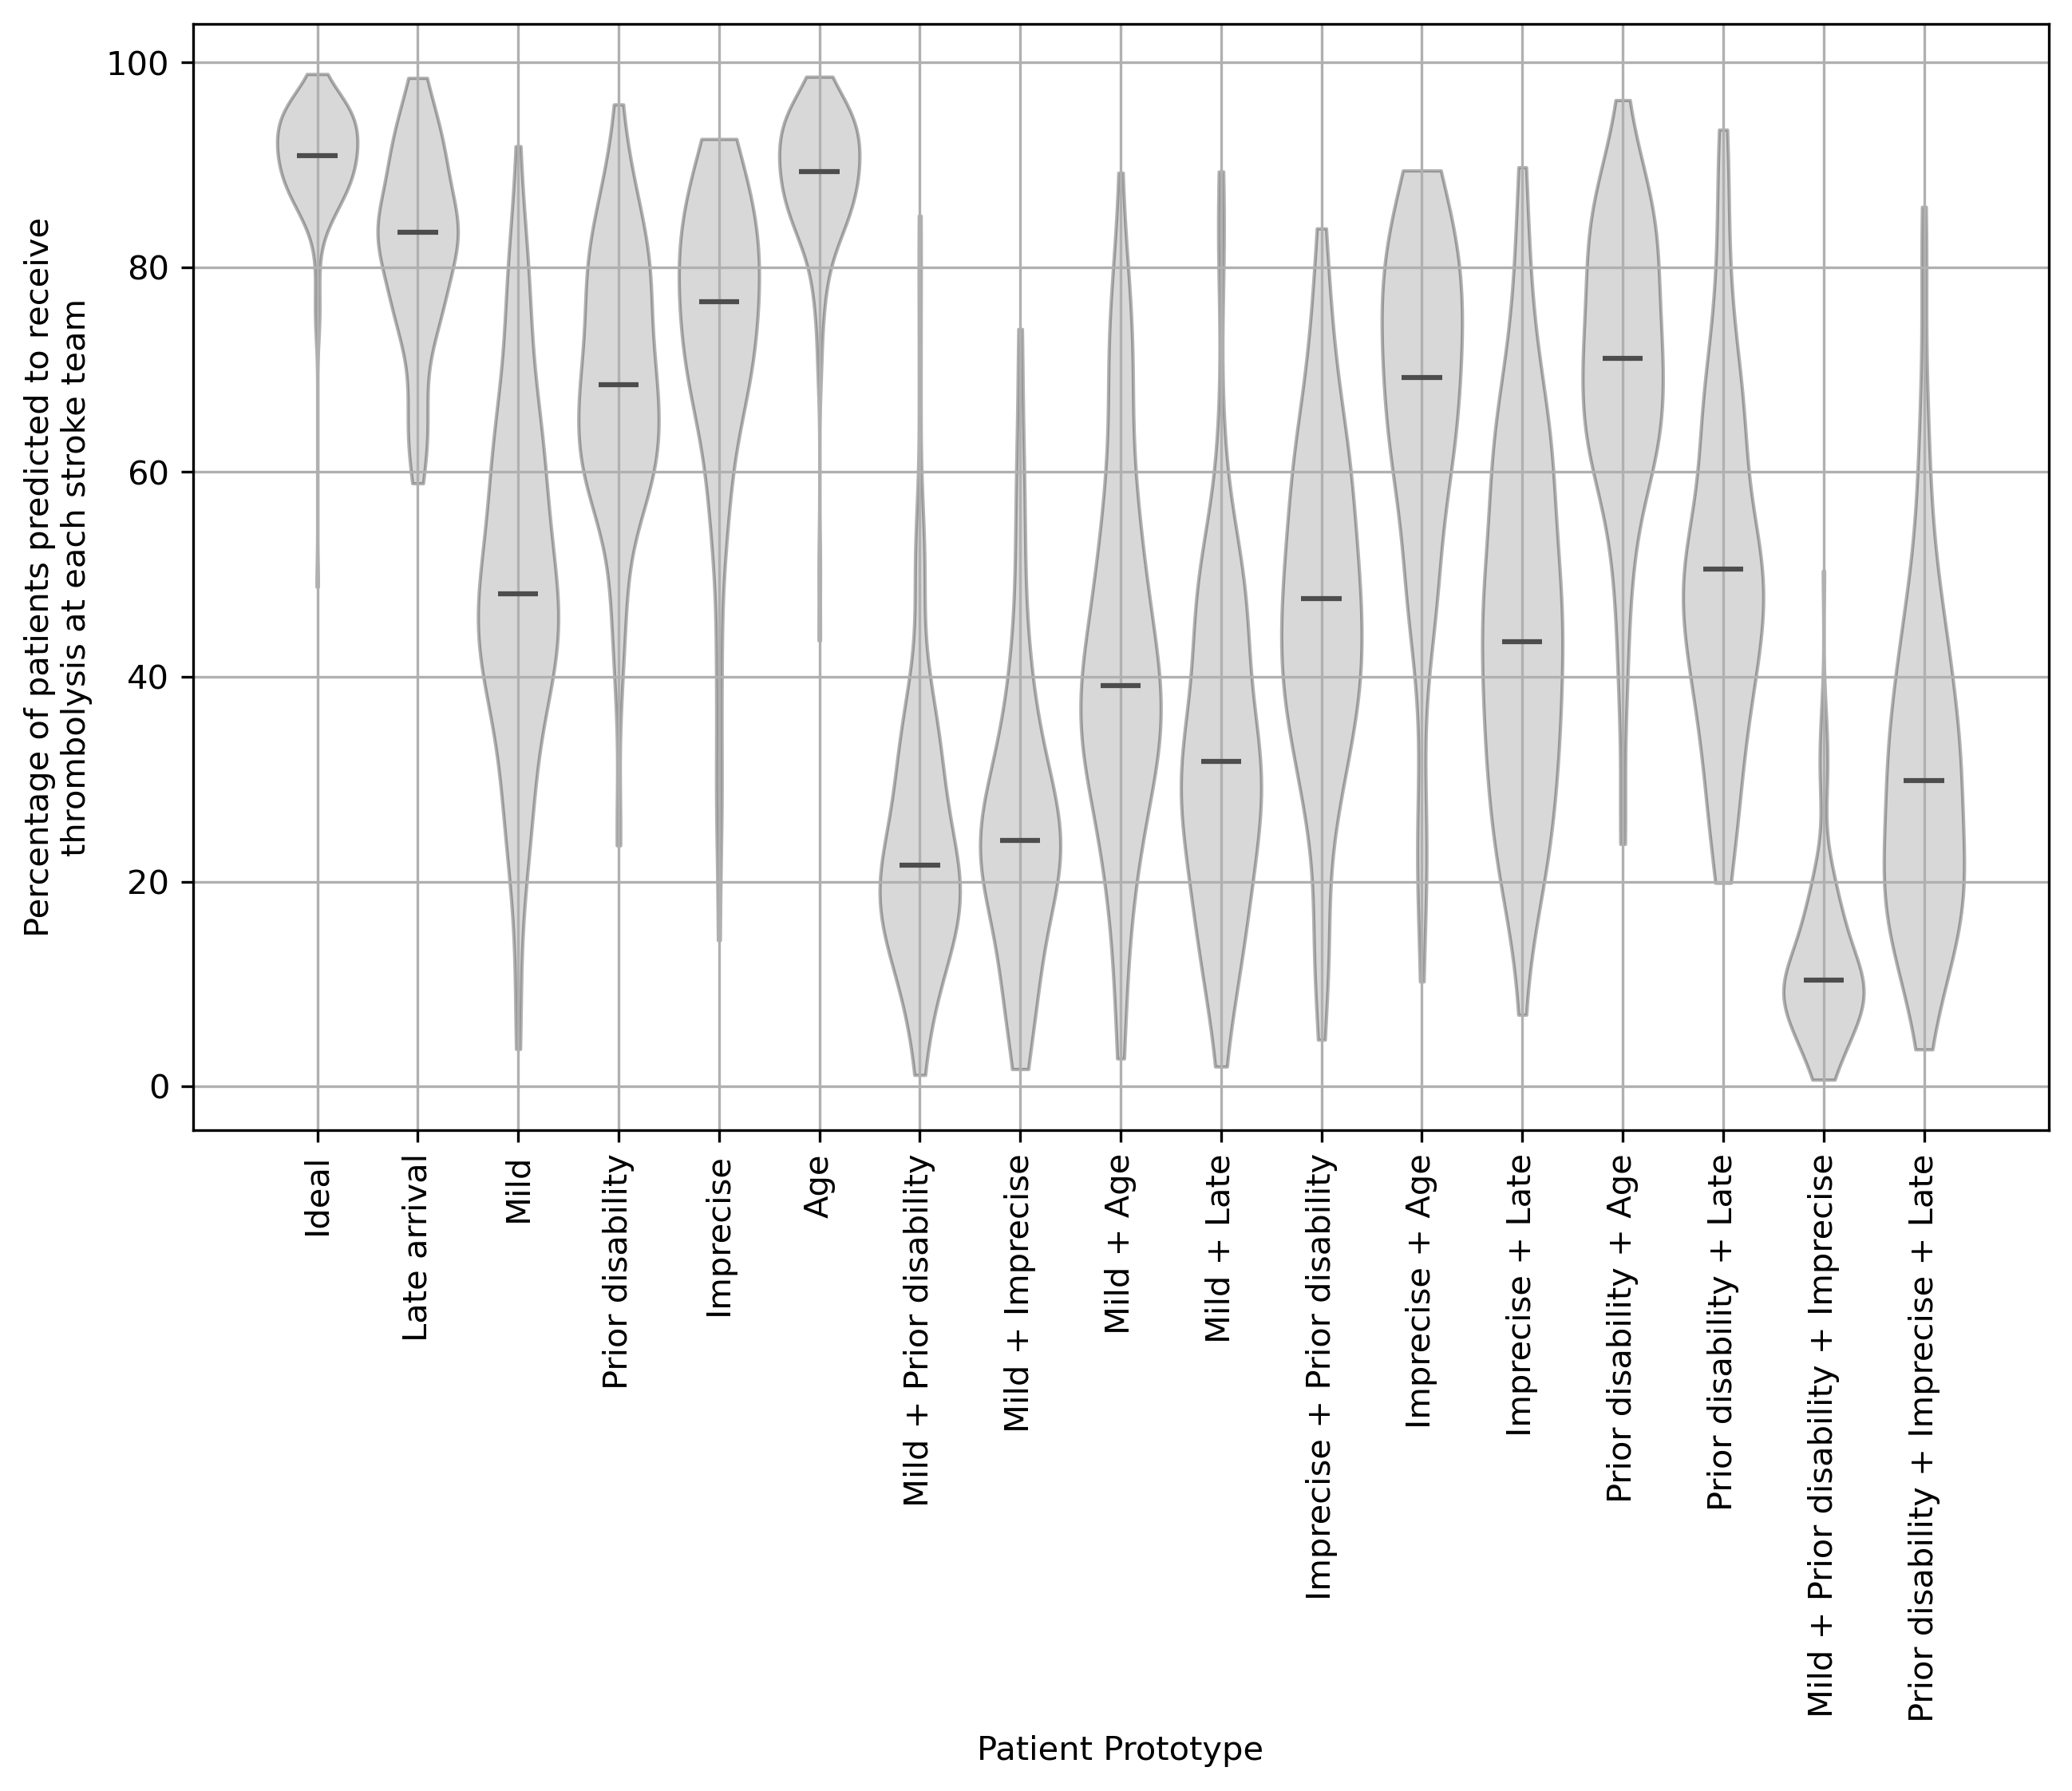
\includegraphics[width=0.75\linewidth]{images/prototype_patients_all_teams}
    \caption{Violin plots showing the variation in predicted thrombolysis rates for 17 patient prototypes across stroke teams. \textit{Ideal}: onset-to-arrival = 90 minutes; arrival-to-scan = 15 minutes; onset-to-thrombolysis = 120 minutes; stroke severity (NIHSS) = 15; pre-stroke disability (mRS) = 0; age = 72.5; precisely known onset; onset not during sleep; stroke type = infarction; patient has no atrial fibrillation and is not receiving anticoagulants for atrial fibrillation; \textit{Late arrival}: as \textit{ideal} but onset-to-arrival = 225 minutes and onset-to-thrombolysis = 255 minutes; \textit{Mild}: As \textit{ideal} but stroke severity = 3; \textit{Prior disability}: as \textit{ideal} but pre-stroke disability = 3; \textit{Imprecise}: as \textit{ideal} but stroke onset time estimated; \textit{Age}: as \textit{ideal} but age = 87.5.}
    \label{fig:thrombolysis_rates_prototype_patients}
\end{figure}

Figure \ref{fig:thrombolysis_rates_prototype_patients_team_x} shows an example of thrombolysis decisions for prototype patients in one stroke team, which is especially unlikely to give thrombolysis to patients with mild stroke, comparing likely use of thrombolysis to \textit{benchmark} hospitals.

\begin{figure}
    \centering
    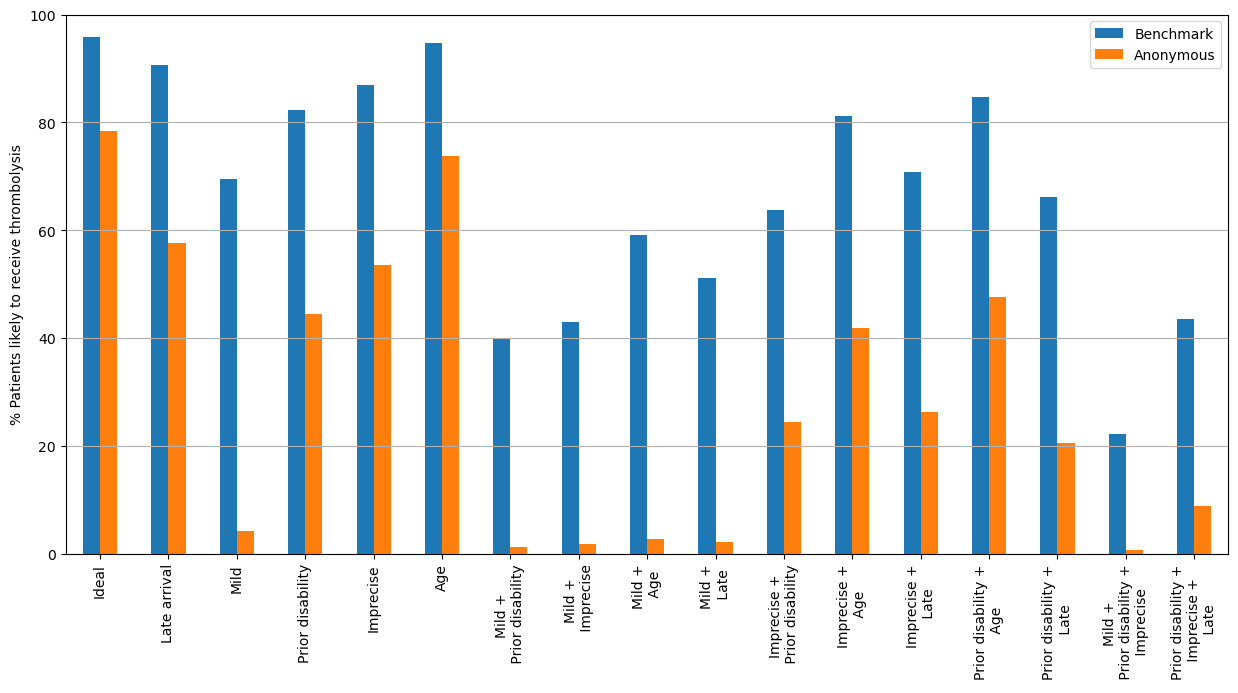
\includegraphics[width=1\linewidth]{images/prototype_patients_team_x.png}
    \caption{Predicted use of thrombolysis in 17 patient prototypes at a single hospital. Results show the the percentage of patients likely to receive thrombolysis, comparing \textit{benchmark decisions} (blue) and decisions likely at the example hospital (orange). Patient prototypes were: \textit{Ideal} candidate characteristics: onset-to-arrival = 90 minutes; arrival-to-scan = 15 minutes; onset-to-thrombolysis = 120 minutes; stroke severity (NIHSS) = 15; pre-stroke disability (mRS) = 0; age = 72.5; precisely known onset; onset not during sleep; stroke type = infarction; patient has no atrial fibrillation and is not receiving anticoagulants for atrial fibrillation. \textit{Late arrival}: as \textit{Ideal} but onset-to-arrival = 225 minutes and onset-to-thrombolysis = 255 minutes; \textit{Mild}: As \textit{Ideal} but stroke severity = 3; \textit{Prior disability}: as \textit{Ideal} but pre-stroke disability = 3; \textit{Imprecise}: as \textit{Ideal} but stroke onset time estimated. \textit{Age}: as \textit{Ideal} but age = 87.5. With combinations of non-ideal features.}
    \label{fig:thrombolysis_rates_prototype_patients_team_x}
\end{figure}


\subsubsection{Expected outcomes in prototype patients}

Figure \ref{fig:example_patient_outcomes} shows examples of outcome prediction for an \textit{ideal} candidate for thrombolysis, and a patient who is otherwise the same but has mild stroke. Expected benefit from thrombolysis may be calculated as the change in the proportion of \textit{good outcomes} (e.g. mRS 0-2), the proportion of \textit{bad outcomes} (e.g. mRS 5-6), or the shift in the central point of the outcome distribution (by weighting each mRS level by the probability of being discharged with that level of disability). 


\begin{figure}[h]
    \centering
    \begin{subfigure}[b]{1.0\textwidth}
        \centering
    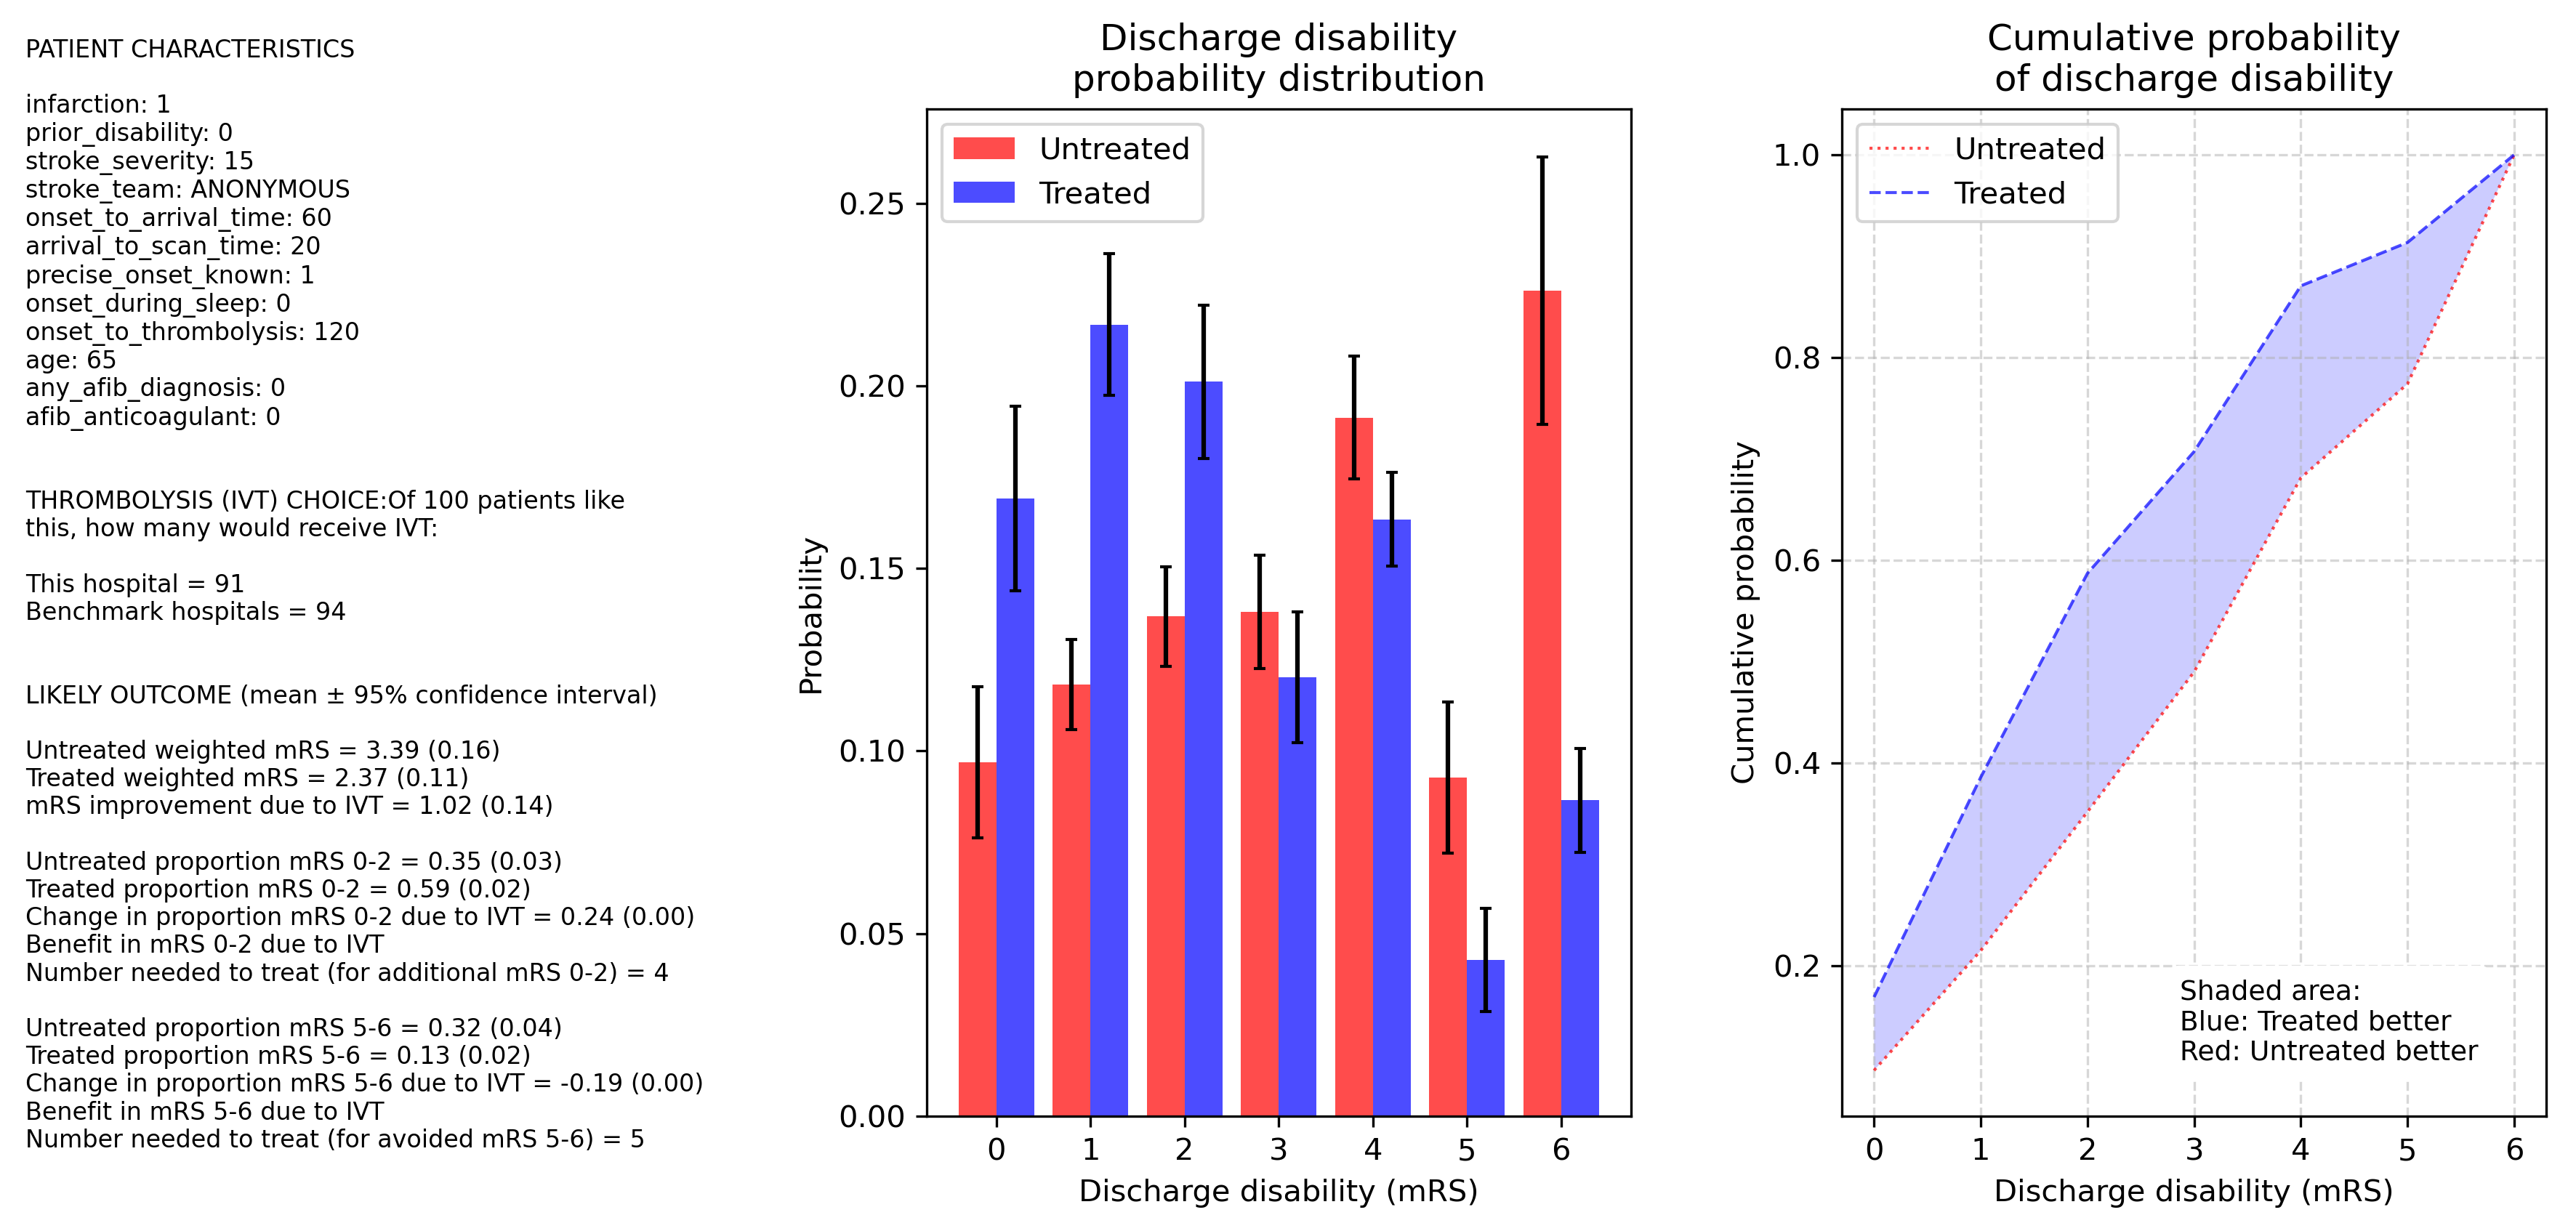
\includegraphics[width=1.0\linewidth]{images/prototype_patient_ideal}
        \caption{\textit{Ideal} candidate for thrombolysis}
        \label{fig:patient_outcome_subfig1}
    \end{subfigure}
    \\
    \vspace{8mm}
    \begin{subfigure}[b]{1.0\textwidth}
        \centering
        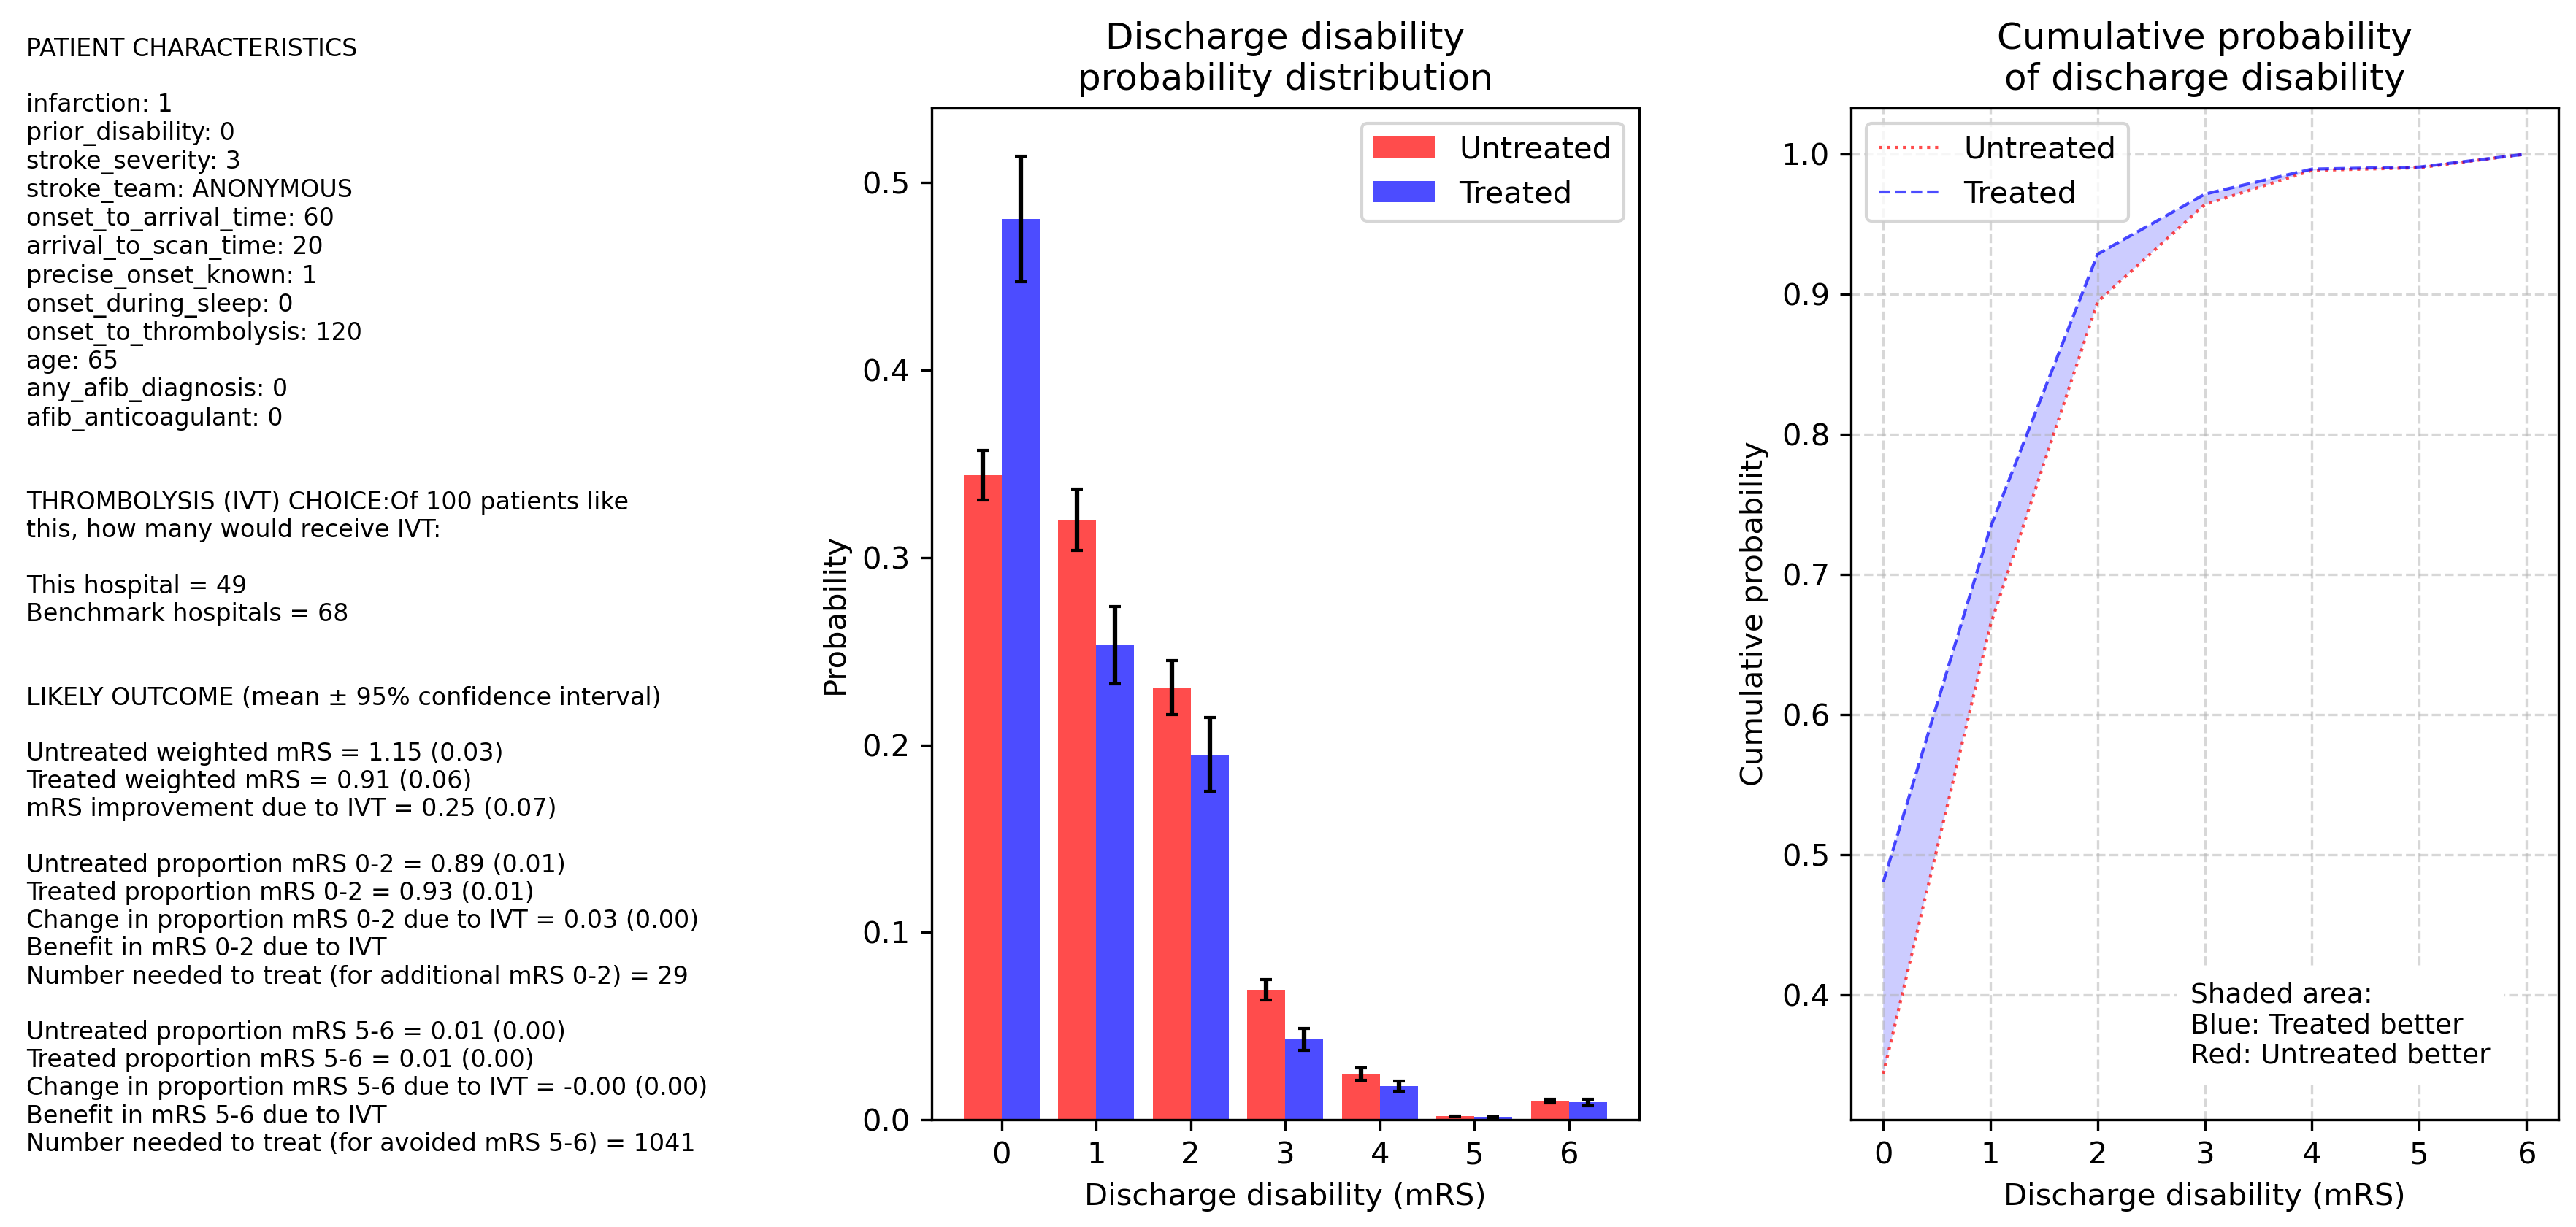
\includegraphics[width=1.0\linewidth]{images/prototype_patient_mild}
        \caption{Patient as \textit{Ideal} candidate for thrombolysis, but with mild stroke (NIHSS 3)}
        \label{fig:patient_outcome_subfig2}
    \end{subfigure}
    \caption{Predicted outcome probabilities, with and without thrombolysis, for an \textit{Ideal} candidate for thrombolysis (top) and for a patient with \textit{mild stroke} (bottom). \textit{Ideal} candidate characteristics: onset-to-arrival = 90 minutes; arrival-to-scan = 15 minutes; onset-to-thrombolysis = 120 minutes; stroke severity (NIHSS) = 15; pre-stroke disability (mRS) = 0; age = 72.5; precisely known onset; onset not during sleep; stroke type = infarction; patient has no atrial fibrillation and is not receiving anticoagulants for atrial fibrillation. Patient with mild stroke is as \textit{Ideal} candidate, but with NIHSS = 3. Errors shown are 95\% confidence limits derived from 30 bootstrapped models.}
    \label{fig:example_patient_outcomes}
\end{figure}



Table \ref{tab:prototype_outcomes} shows predicted outcomes across all prototype patients. All these patients would likely benefit from thrombolysis, but the benefit in mild stroke was smaller.

\begin{minipage}{1\textwidth}
\small
\begin{longtable}{p{5.2cm} | p{1.6cm} p{1.6cm} p{1.5cm} | p{1.6cm} p{1.6cm} p{1.5cm}}
\caption{Predicted outcomes for patient prototypes. \textit{Ideal}: onset-to-arrival = 90 minutes; arrival-to-scan = 15 minutes; onset-to-thrombolysis = 120 minutes; stroke severity (NIHSS) = 15; pre-stroke disability (mRS) = 0; age = 72.5; precisely known onset; onset not during sleep; stroke type = infarction; patient has no atrial fibrillation and is not receiving anticoagulants for atrial fibrillation. \textit{Late arrival}: as \textit{Ideal} but onset-to-arrival = 225 minutes and onset-to-thrombolysis = 255 minutes; \textit{Mild}: As \textit{Ideal} but stroke severity = 3; \textit{Prior disability}: as \textit{Ideal} but pre-stroke disability = 3; \textit{Imprecise}: as \textit{ideal} but stroke onset time estimated. \textit{Age}: as \textit{Ideal} but age = 87.5. Results show probability-weighted disability at discharge, and the proportion of patients predicted to have a very poor outcome (mRS 5-6). With combinations of non-ideal characteristics.}\\
\label{tab:prototype_outcomes}
Patient prototype & Untreated probability-weighted mRS & Treated probability-weighted mRS & Improve-ment & Untreated proportion mRS 5-6 & Treated proportion mRS 5-6 & Improve-ment\\
\endhead
\midrule
Ideal & 3.39 & 2.37 & 1.02 & 0.32 & 0.13 & 0.19\\
Late & 3.39 & 2.73 & 0.66 & 0.32 & 0.18 & 0.14\\
Mild & 1.15 & 0.91 & 0.23 & 0.01 & 0.01 & 0.00\\
Prior disability & 4.22 & 3.61 & 0.61 & 0.41 & 0.23 & 0.19\\
Imprecise & 3.49 & 2.39 & 1.10 & 0.33 & 0.13 & 0.20\\
Age & 4.22 & 3.51 & 0.71 & 0.50 & 0.35 & 0.16\\
Mild + Prior disability & 2.92 & 2.60 & 0.32 & 0.04 & 0.04 & 0.00\\
Mild + Imprecise & 1.28 & 1.01 & 0.26 & 0.02 & 0.01 & 0.00\\
Mild + Age & 1.84 & 1.63 & 0.22 & 0.04 & 0.03 & 0.01\\
Mild + Late & 1.15 & 0.77 & 0.39 & 0.01 & 0.00 & 0.00\\
Imprecise + Prior disability & 4.33 & 3.67 & 0.66 & 0.44 & 0.24 & 0.20\\
Imprecise + Age & 4.31 & 3.57 & 0.74 & 0.53 & 0.36 & 0.17\\
Imprecise + Late & 3.49 & 2.75 & 0.74 & 0.33 & 0.17 & 0.17\\
Prior disability + Age & 4.62 & 4.35 & 0.27 & 0.53 & 0.44 & 0.08\\
Prior disability + Late & 4.22 & 3.70 & 0.52 & 0.41 & 0.27 & 0.14\\
Mild + Prior disability + Imprecise & 3.01 & 2.65 & 0.36 & 0.06 & 0.06 & 0.00\\


\end{longtable}
\normalsize
\end{minipage}

\subsection{Mild stroke}

Table \ref{tab:mild_stroke} shows the predicted benefit of thrombolysis, for those who actually received thrombolysis, in mild ischaemic stroke (NIHSS 0-4) and non-mild stroke (NIHSS 5+) at \textit{benchmark hospitals} and \textit{non-benchmark hospitals}. In those mild stroke patients who actually received thrombolysis, either at a benchmark hospital or a non-benchmark hospital, it was predicted that there would be an increased proportion of good outcomes, and a beneficial shift in average mRS, but that there would be a small increase in bad outcomes. For non-mild stroke, thrombolysis improved by all outcome measures.

\begin{minipage}{1\textwidth}
\small
\renewcommand{\arraystretch}{1.2}
\begin{longtable}{p{7.2cm} | p{1.6cm} p{1.6cm} | p{1.6cm} p{1.6cm}}
\caption{Patient characteristics and predicted outcomes for mild stroke (NIHSS 0-4) and non-mild stroke (NIHSS 5+). Results shown are the mean for all patients who actually received treatment at either a non-benchmark hospital or a benchmark hospital.}\\
\label{tab:mild_stroke}

Metric & Non-benchmark NIHSS 0-4 & Non-benchmark NIHSS 5+ & Benchmark NIHSS 0-4 & Benchmark NIHSS 5+\\
\endhead
\midrule
Stroke severity & 3.1 & 12.8 & 2.9 & 12.5\\
Onset to thrombolysis (minutes) & 147 & 138 & 140 & 130\\
Proportion onset known precisely & 86\% & 84\% & 77\% & 71\%\\
Proportion untreated mRS 0-1 & 0.556 & 0.240 & 0.564 & 0.234\\
Proportion untreated mRS 0-2 & 0.797 & 0.401 & 0.795 & 0.399\\
Proportion untreated mRS 5-6 & 0.026 & 0.281 & 0.024 & 0.284\\
Untreated weighted mRS & 1.535 & 3.188 & 1.537 & 3.205\\
Change in proportion mRS 0-1 (+ve is better) & 0.019 & 0.063 & 0.027 & 0.072\\
Change in proportion mRS 0-2 (+ve is better) & 0.012 & 0.079 & 0.009 & 0.078\\
Change in proportion mRS 5-6 (-ve is better) & 0.010 & -0.056 & 0.009 & -0.057\\
Change in weighted mRS ( -ve is better) & -0.036 & -0.341 & -0.053 & -0.354\\

\end{longtable}
\normalsize
\end{minipage}


\subsection{Lifetime economic model}

Table \ref{tab:health_econ} shows the modelled health economics of thrombolysis use, comparing actual use of thrombolysis with \textit{benchmark} thrombolysis use. The effect of thrombolysis was estimated by predicting the outcomes with and without thrombolysis for the two groups (those that actually received thrombolysis, and those predicted to receive thrombolysis using \textit{benchmark} decisions). Benchmark decisions maintain the benefit of using thrombolysis, but extend that benefit to more patients. This extended benefit was not at the cost of any predicted increase in the worst outcomes (mRS 5-6). The extended benefit led to more QALYs added across the population by treatment, and more predicted savings to NHS healthcare costs.

\begin{table}[!h]
\small
\caption{Health economic analysis: Analysis for  populations based on predicted benefit (or dis-benefit) of thrombolysis. The effect of thrombolysis was estimated by predicting the outcomes with and without thrombolysis for the two groups (those that actually received thrombolysis, and those predicted to receive thrombolysis using \textit{benchmark} decisions). The analysis compares the populations currently treated, or the population that would be treated using \textit{benchmark} decisions (the majority vote of the predicted choice of the the 25 stroke teams most likely to use thrombolysis). Results are shown for (a) the treated populations, and (b) adjusted for 1,000 emergency stroke admissions }
\label{tab:main}

\begin{subtable}{1\textwidth}
\centering
\caption{Analysis of the predicted effect of thrombolysis in two population subgroups: 1) those patients who actually received thrombolysis, or 2) those patients where the \textit{benchmark decision} would be to use thrombolysis. For each populations the outcomes with and without thrombolysis were predicted.}
\begin{tabular}{p{2.0cm} p{1.5cm} p{1.2cm} p{1.3cm} p{1.5cm} p{1.3cm} p{1.4cm} p{1.3cm} p{1.3cm}}
\toprule
Modelled population & \raggedright Modelled treatment & Death & Survival (median years) & Care years (median) & QALYs & \raggedright Discounted cost per patient & Proportion mRS 0-2 & Proportion mRS 5-6\tabularnewline
\midrule
Actual use & Untreated & 17.1\% & 7.60 & 0.28 & 5.020 & £20,370 & 47.1\% & 23.9\%\tabularnewline
& Treated & 14.2\% & 7.91 & 0.25 & 5.258 & £19,806 & 53.9\% & 19.3\%\tabularnewline
& Difference & -2.9\% & 0.31 & -0.03 & 0.238 & -£565 & 6.8\% & -4.7\%\tabularnewline
\midrule
Benchmark & Untreated & 17.4\% & 7.63 & 0.28 & 5.036 & £20,388 & 46.5\% & 24.1\%\tabularnewline
& Treated & 14.4\% & 7.93 & 0.25 & 5.269 & £19,784 & 53.4\% & 19.4\%\tabularnewline
& Difference & -3.0\% & 0.30 & -0.03 & 0.234 & -£603 & 6.9\% & -4.8\%\tabularnewline

\end{tabular}
\end{subtable}

\vspace{3mm}

\begin{subtable}{1\textwidth}
\centering
\caption{Analysis for 1,000 emergency stroke admissions (all stroke types)}
\begin{tabular}{p{1.9cm} p{1.9cm} p{1.9cm} p{1.9cm} p{1.9cm} p{1.9cm} p{2.2cm}}
\toprule
Modelled population & Proportion treated & QALYs added & Healthcare costs saved & \raggedright Thrombolysis cost (£450 per patient) & \raggedright Cost per QALY added & \raggedright Net cost of thrombolysis\tabularnewline
\midrule
Actual & 11.0\% & 26.3 & £62,294 & £49,658 & £1,890 & -£12,637\tabularnewline
Benchmark & 13.6\% & 31.7 & £81,914 & £61,117 & £1,927 & -£20,797\tabularnewline
\bottomrule
\end{tabular}
\end{subtable}
\label{tab:health_econ}
\end{table}

\normalsize

\subsection{Pathway model}

Figure \ref{fig:thrombolysis_rates_teams} compares observed and predicted thrombolysis use (based on historic performance, and applying \textit{benchmark decisions}). Predicted and observed thrombolysis use correlate very closely (r-squared 0.94). Predicted rates were, on average, slightly higher (1.7\%) than observed rates.

\begin{figure}[!h]
    \centering
    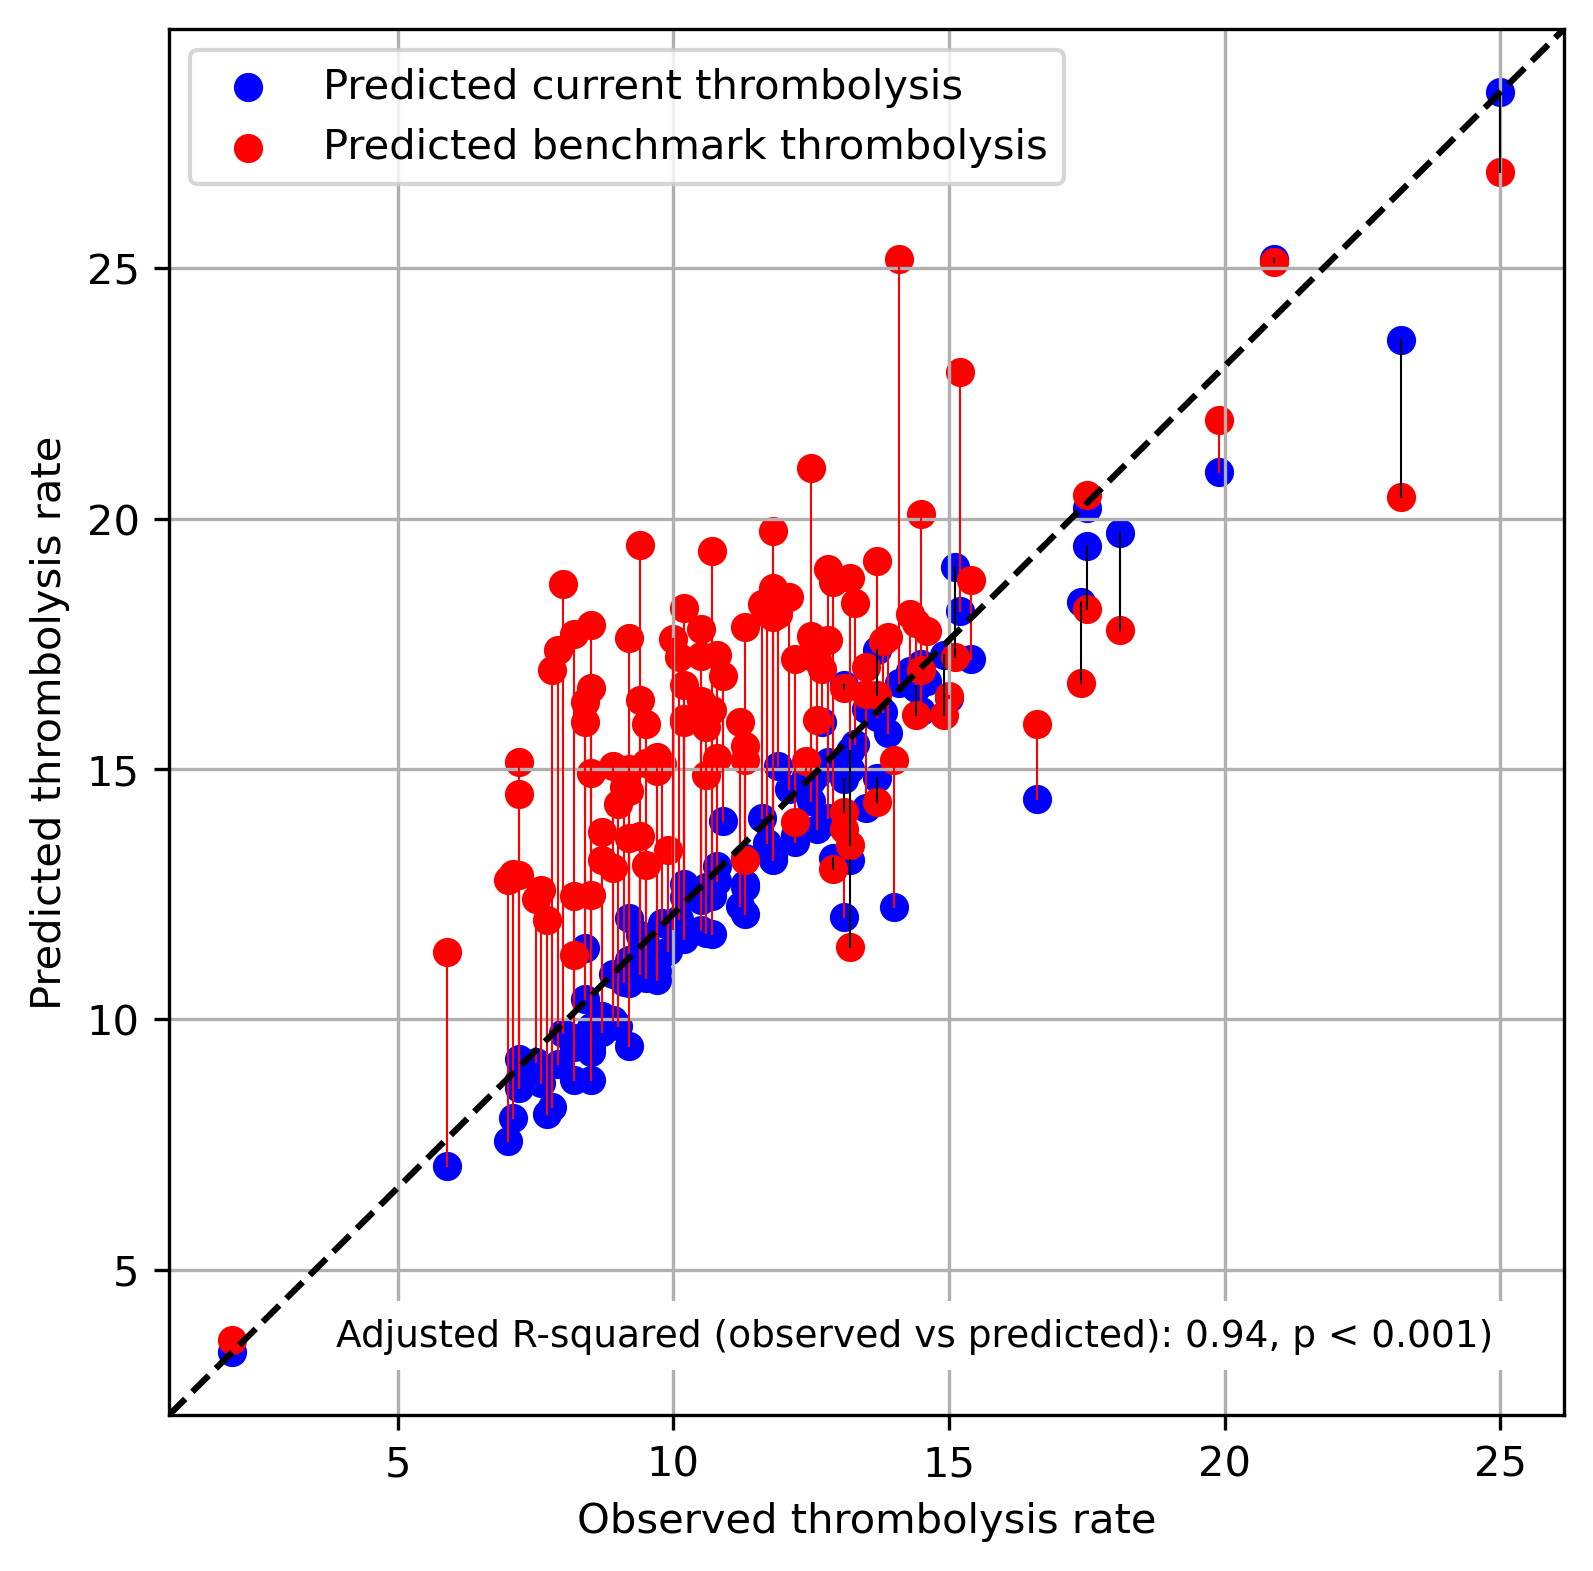
\includegraphics[width=0.5\linewidth]{images/thrombolysis_rates_model}
    \caption{Comparison of observed and predicted thrombolysis use across stroke teams. Blue circles show predictions based on historic hospital performance. Red circles show the expected thrombolysis use if \textit{benchmark decisions} were made. The black dotted line shows least-squares regression analysis between observed and predicted (using historic performance) thrombolysis use.}
    \label{fig:thrombolysis_rates_teams}
\end{figure}


Across the study population, by combining pathway improvements, thrombolysis use in all those emergency stroke admissions arriving by ambulance shows the potential to be increased from 13\% to 20\% (figure \ref{fig:scenarios_population}). Using a model based on clinical trial data, benefit, as measured by number of number of people discharged with no, or minimal, disability (mRS 0 or 1) could be doubled from 10 to 20 additional excellent outcomes per 1,000 admissions. The single most influential change was applying \textit{benchmark} decisions. Improving speed would not significantly increase the number of people given thrombolysis, but would lead to more benefit from thrombolysis (as all treated patients will have improved benefit). Figure \ref{fig:scenarios_team} shows this analysis applied to a single stroke team.


\begin{figure}[!h]
    \centering
    \begin{subfigure}[b]{1\textwidth}
        \centering
        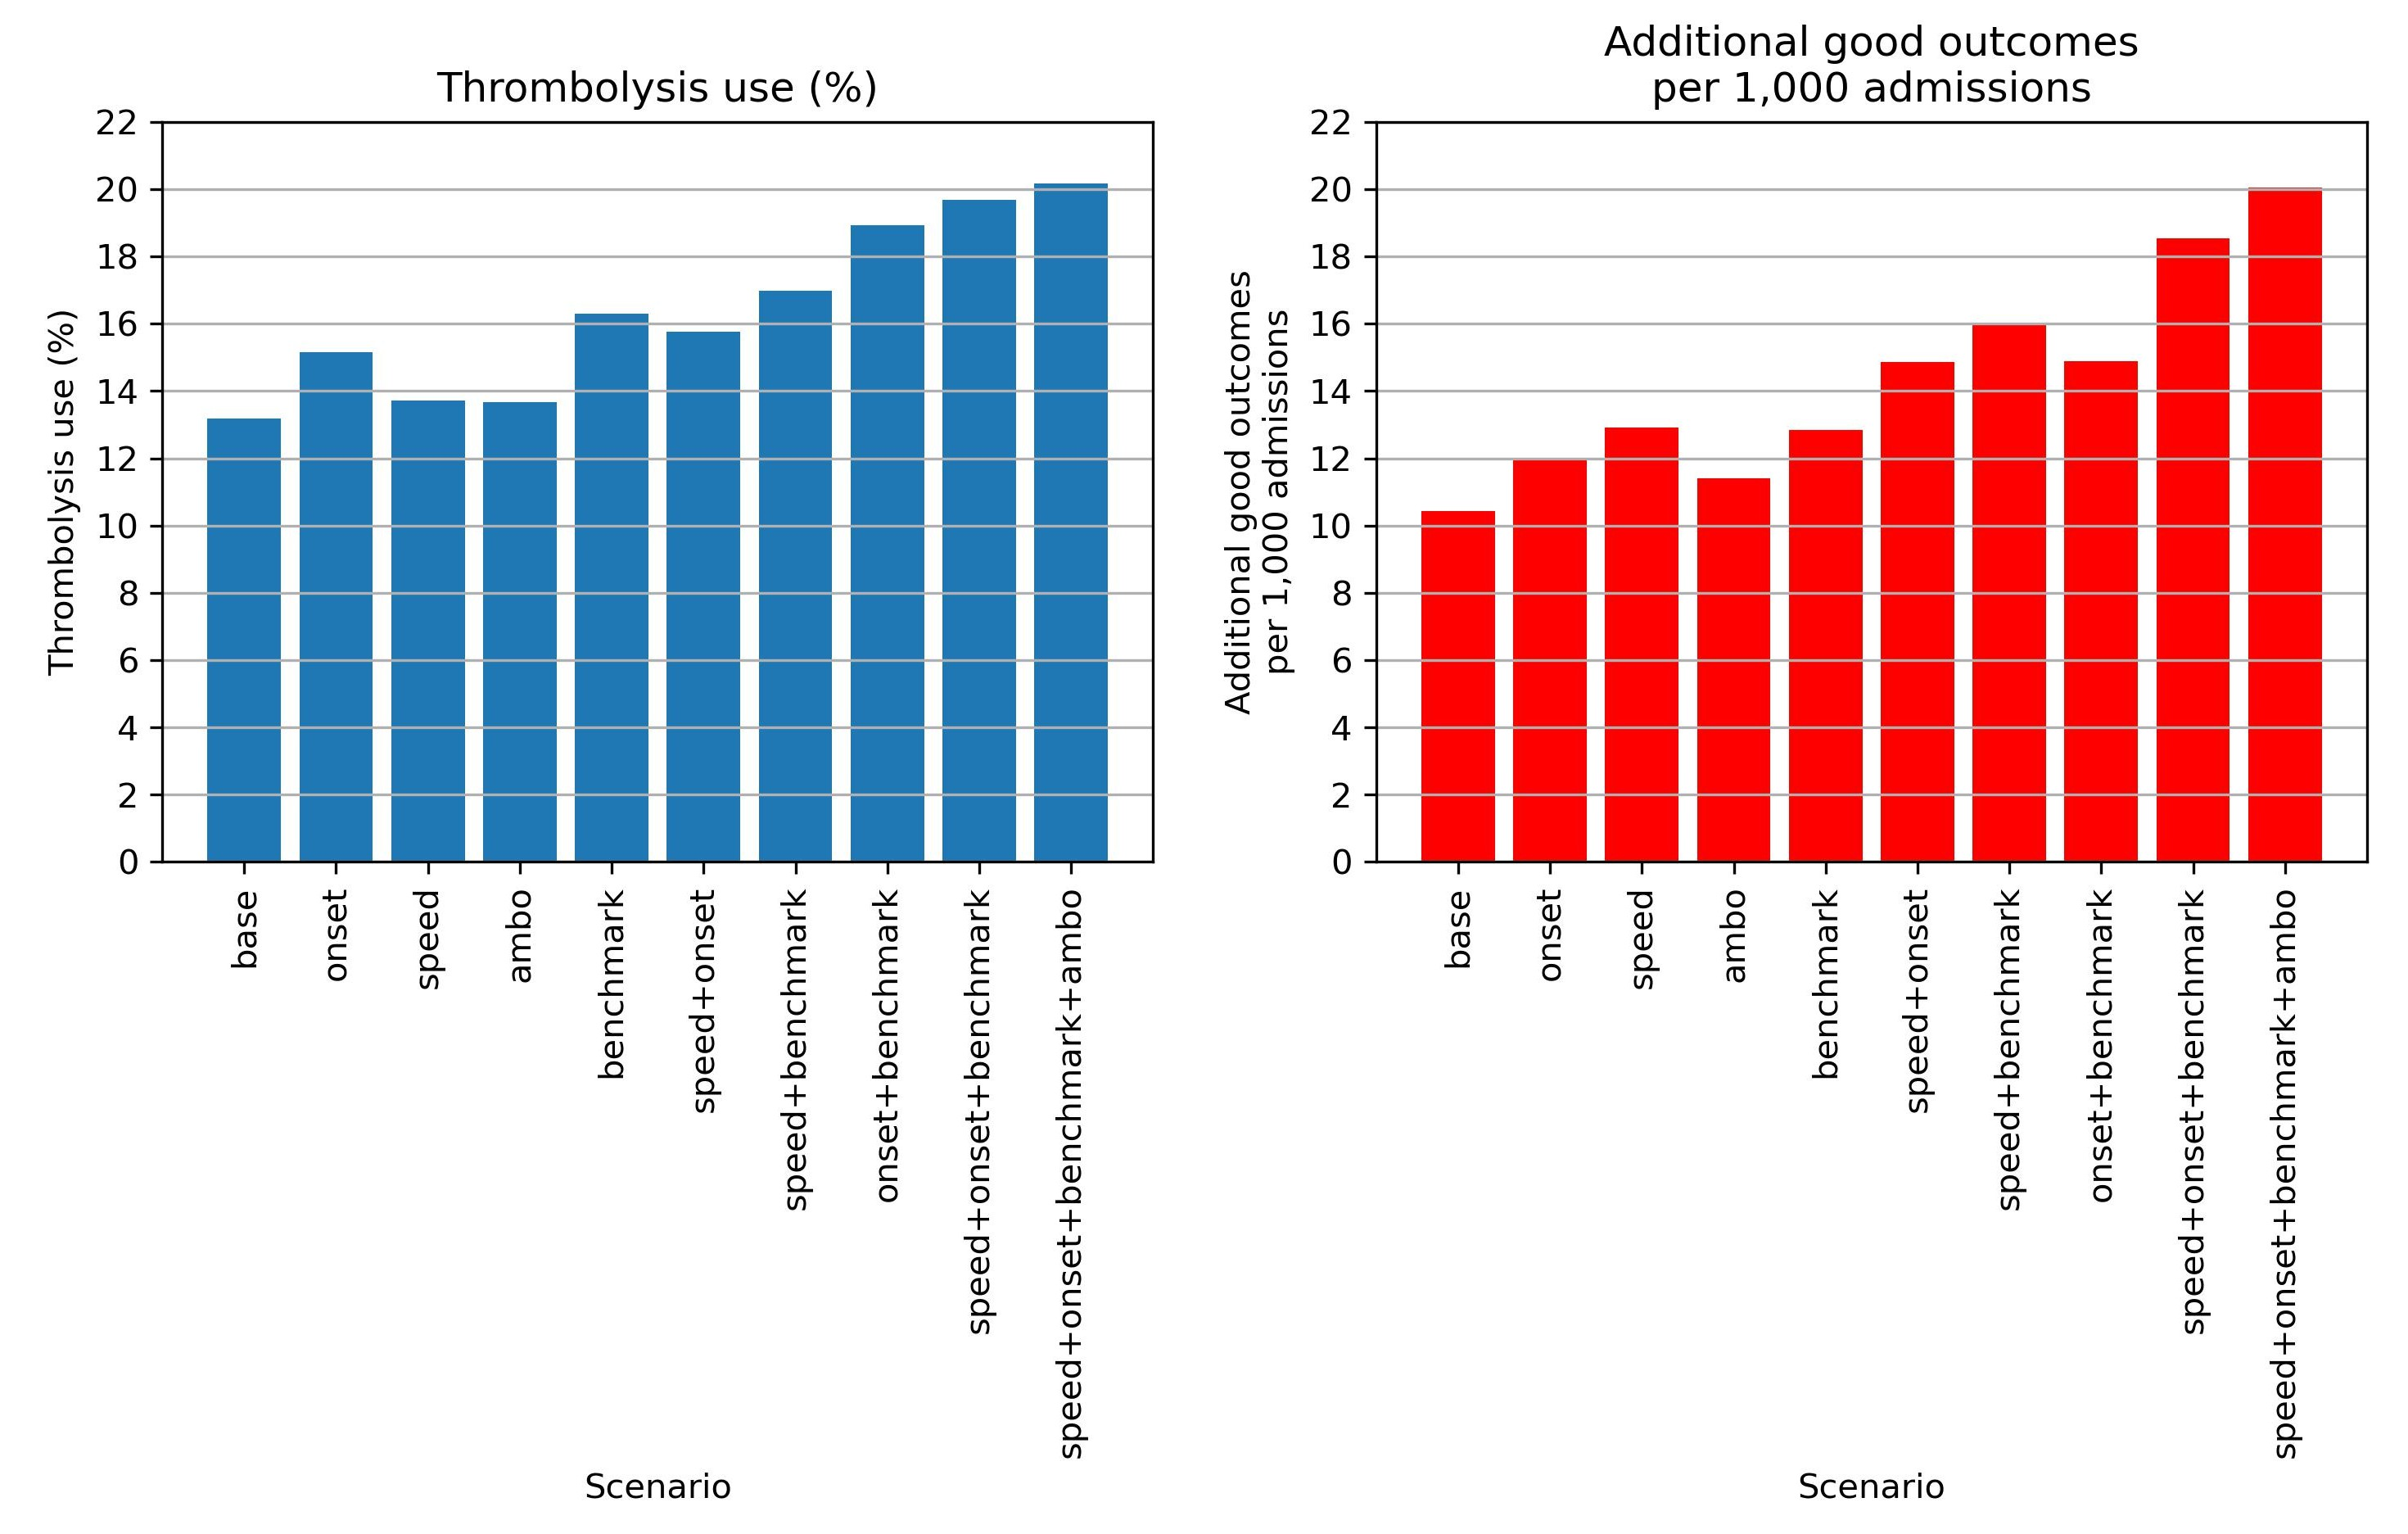
\includegraphics[width=0.8\linewidth]{images/sim_results_summary}
        \caption{Changes across the study population}
        \label{fig:scenarios_population}
    \end{subfigure}
    \\
    \vspace{8mm}
    \begin{subfigure}[b]{1\textwidth}
        \centering
    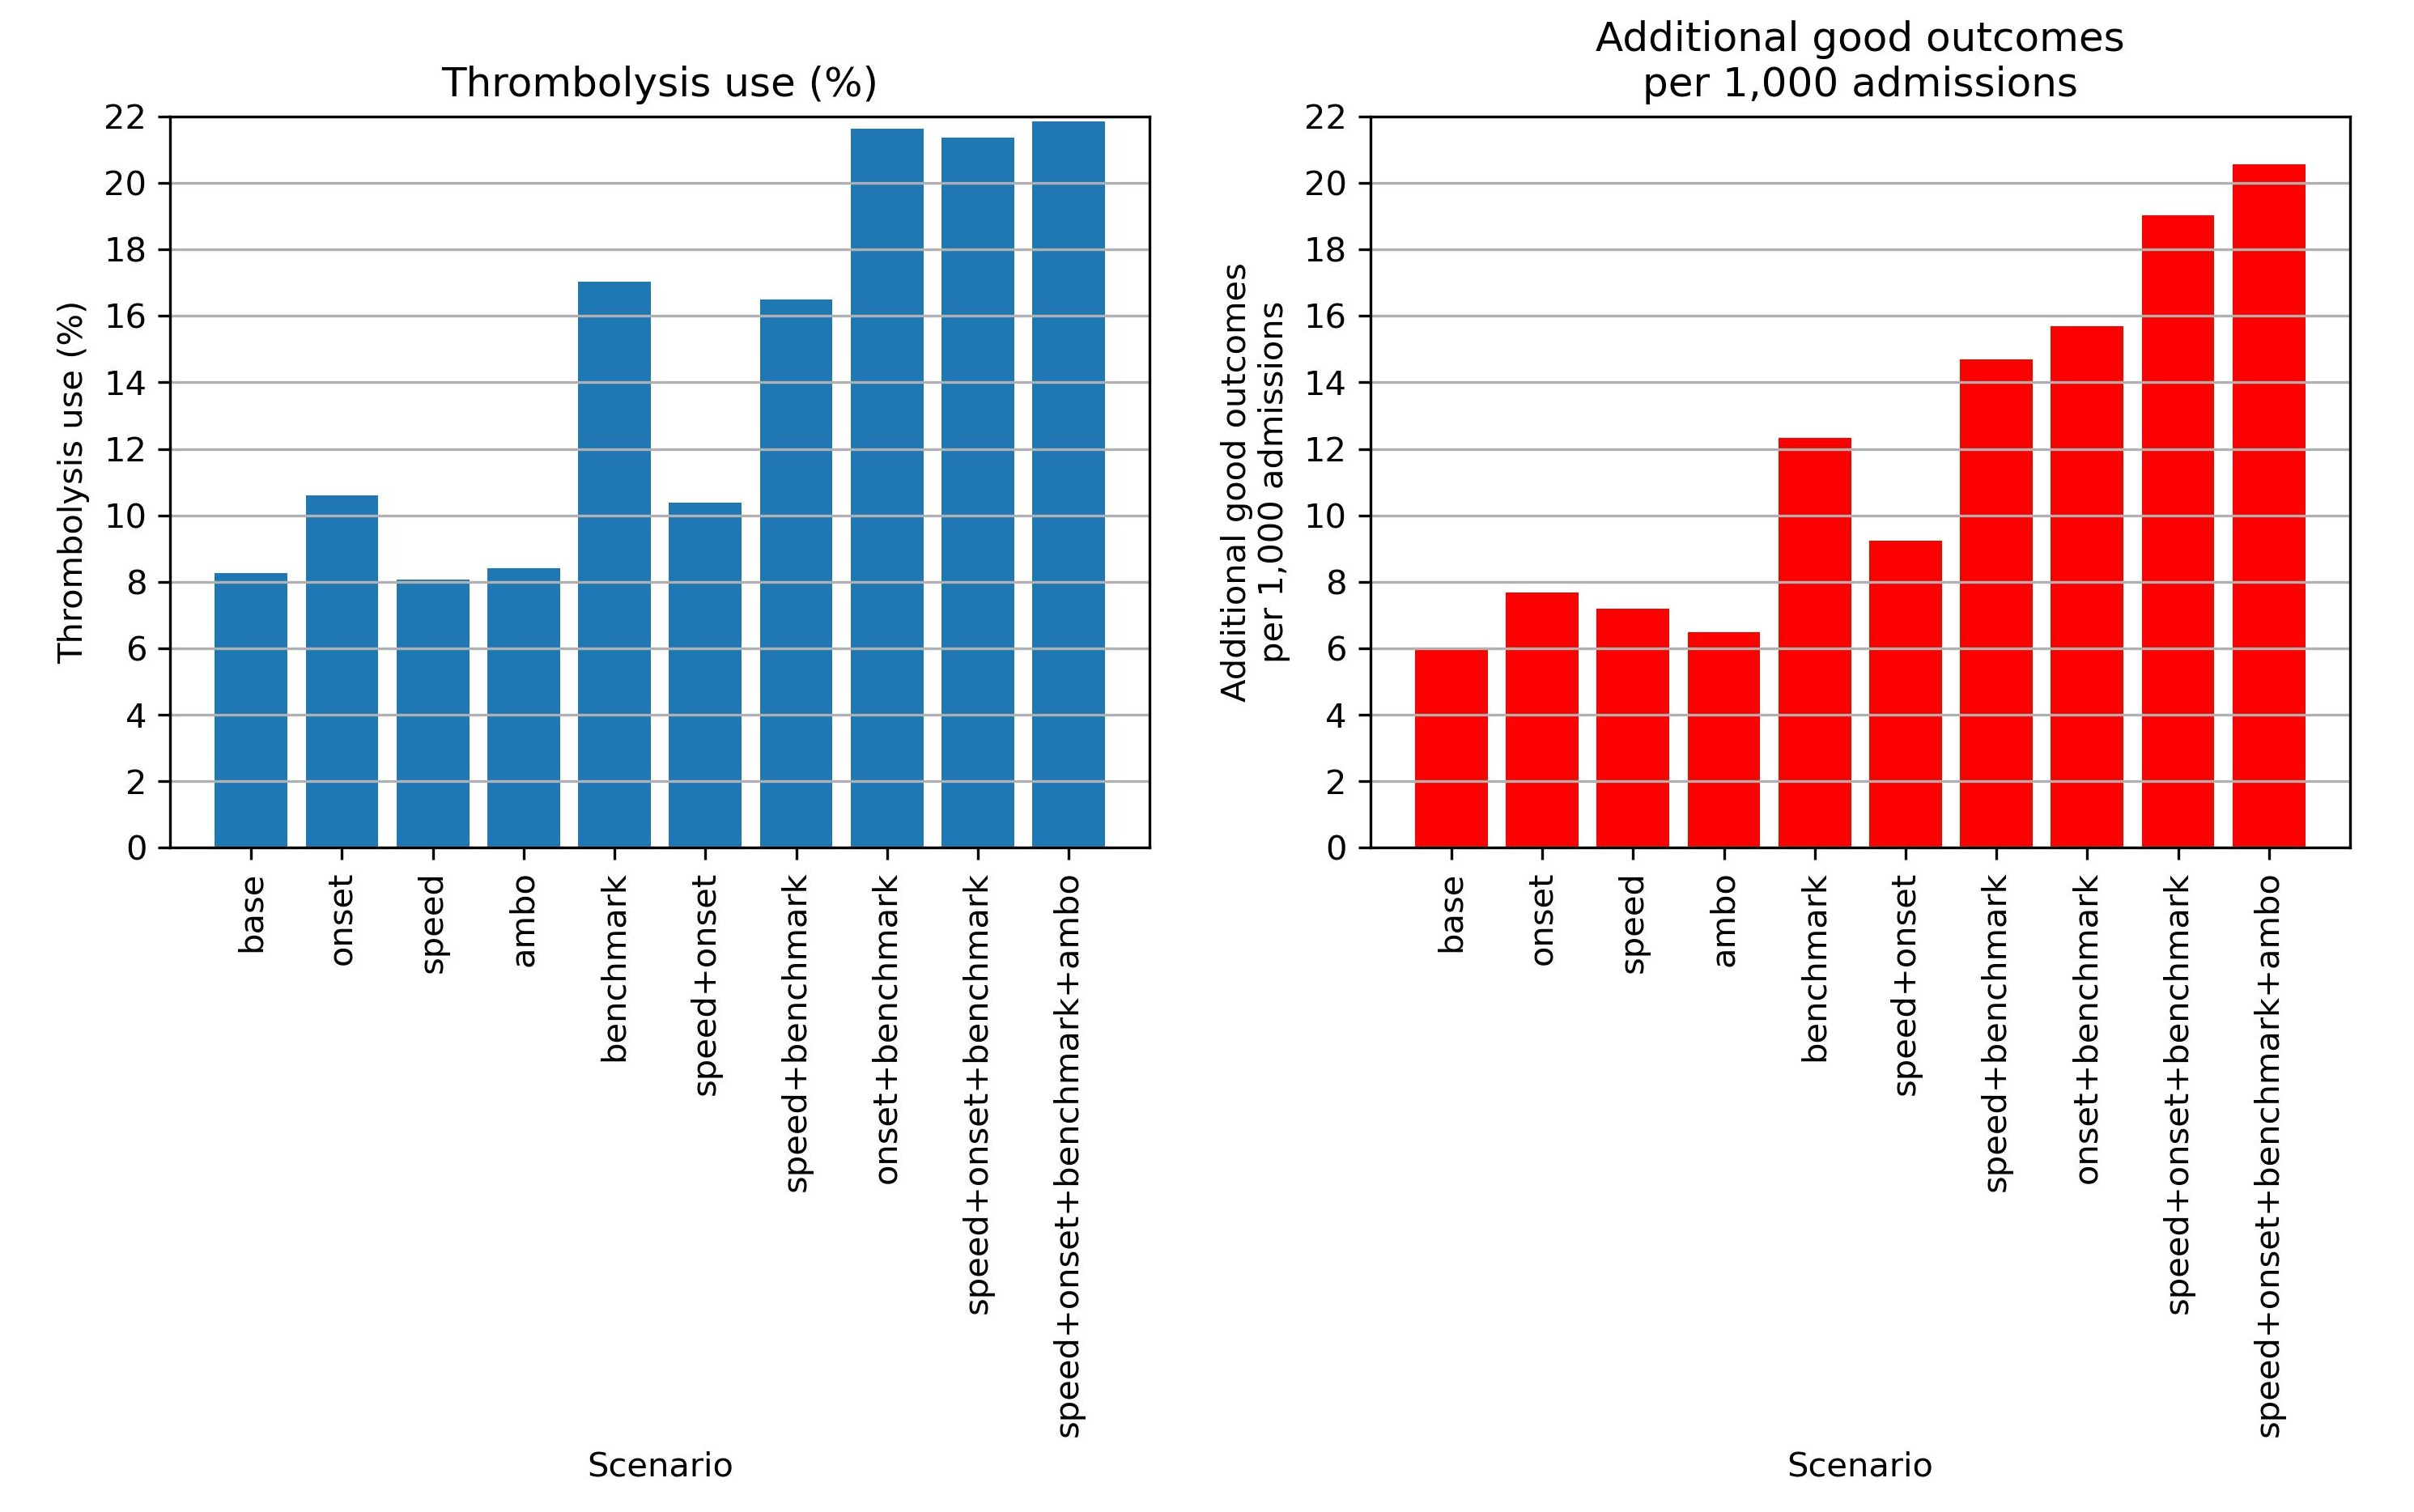
\includegraphics[width=0.8\linewidth]{images/sim_results_team_x}
        \caption{Changes in one stroke team}
        \label{fig:scenarios_team}
    \end{subfigure}
    \caption{Expected effect of alternative process improvement initiatives across the study population (top) or one specific stroke team (bottom). Each chart shows the effect on thrombolysis use (left) and on number of additional good outcomes (mRS 0-1) per 1,000 admissions due to use of thrombolysis (right). \textit{Base}: Uses the hospitals’ recorded pathway statistics. \textit{Onset}: Sets the proportion of patients with a known stroke onset time to the national upper quartile (79.6\%) if currently less than the national upper quartile. \textit{Speed}: Sets 95\% of patients having a scan within 4 hours of arrival, and all patients have 15 minutes arrival-to-scan time and 15 minutes scan-to-needle time. \textit{Ambo}: Subtracts 15 minutes from the current ambulance call to arrival-at-hospital times. \textit{Benchmark}: The benchmark thrombolysis rate takes the likelihood to give thrombolysis for patients scanned within 4 hours of onset from the majority vote of the 25 benchmark hospitals.}
    \label{fig:sim_results_summary}
\end{figure}



\section{Discussion}

Thrombolysis use in England and Wales is highly variable between stroke teams, and falls well short of NHS England's target of 20\% emergency stroke admissions, and is much lower overall than the European average (15\% of all stroke \cite{aguiar_de_sousa_delivery_2023}). Previously we have identified that hospital processes and decision-making cause more variation than differences in patient populations. A significant amount of variation comes from clinician's enthusiasm to use thrombolysis \cite{allen_use_2022, allen_using_2022}. In that earlier work, we developed methods to compare decision-making between stroke teams. We subsequently added an explainability model to the predictions \cite{pearn_what_2023}, and we were able to identify factors that affected choice of thrombolysis and showed that almost all stroke teams would normally give thrombolysis to \textit{ideal} candidates for thrombolysis (e.g. a patient with moderate-severe stroke, no prior disability, thrombolysis would given in 2 hours, age under 80) but stroke teams varied in their use of thrombolysis in patients with non-ideal characteristics. In associated qualitative work, we found that while clinicians would be influenced by understanding the practice of other clinicians, they also wanted the machine learning modelling expanded to predict outcomes to ensure that higher thrombolysing units were doing more good than harm \cite{allen_using_2022}. In the work we describe here we have addressed outcomes. The work described here is companion work to in-depth studies on how the observed effect of thrombolysis compares with clinical trials \cite{pearn_thrombolysis_2024} and a study on whether those receiving thrombolysis are the the ones who will most likely benefit from it \cite{pearn_are_2024}. Using simplified models compared to our first work, we were also able to construct \textit{prototype patients} to exemplify variation in thrombolysis use and outcomes. We also used the disability-level outcomes of the machine learning model as the input to a health economics model to evaluate the cost-effectiveness of thrombolysis from observational data on use of thrombolysis.

\textit{Prototype patients} showed how non-ideal characteristics of a candidate for thrombolysis affected stroke teams' willingness to use thrombolysis. The largest variation in use came with mild stroke patients and those patients with prior disability. When considering overall use of thrombolysis, use in mild stroke patients will be very influential as mild stroke (NIHSS 0-4) make up 53\% of the general emergency stroke population, though they made up less than 10\% of the clinical trial population \cite{emberson_effect_2014}. Our analysis showed that patients with mild stroke could still benefit from thrombolysis, but the benefit is smaller than in more severe stroke (as there is less room for improvement) and is dependent on other patient features. An analysis of admitted mild stroke patients (rather than prototype patients) showed that those mild stroke patients actually receiving thrombolysis are predicted to have improved outcomes when measured as the proportion of mRS 0-1 or mRS 0-2, or the average disability outcome, but with a small increase (no more than 1\% absolute risk increase) in risk of the worst outcomes (mRS 5-6). Other studies \cite{romano_predictors_2021, coutts_tenecteplase_2024} reported no net benefit, or net harm, of thrombolysis in patients with mild stroke (NIHSS 0-5). Our models predict benefit is present in some, but not all, patients with mild stroke, and overall those receiving thrombolysis (or would receive thrombolysis at the \textit{benchmark stroke teams} with higher thrombolysis use), are receiving a net improvement in outcomes (measured as shift in mRS).  Further work to investigate and inform guidelines around use of thrombolysis in mild stroke could be beneficial.

Our models also indicate that teams also varied in their attitude to use of thrombolysis in patients with prior disability. Though the existence of prior disability limits the improvement possible with thrombolysis, our machine learning identified that there was still significant benefit to be had from thrombolysis. Patients with significant prior disability were excluded from the landmark trials of thrombolysis, but our outcome-based analysis of a large, prospective real-world observational registry would suggest that these patients stand to benefit to the same extent as those without prior disability - reassuring clinicians that this extension to the strict eligibility criteria of the original trials is still resulting in substantial net benefit and cost-effectiveness. 

A third area where stroke teams differ is willingness to use thrombolysis in patients with an estimated rather than precise onset time. Our modelling suggests that outcomes when the onset time is estimated, rather than known precisely, is the same or slightly better (for any assumed onset-to-thrombolysis time) than with a precisely known onset time. The slight improvement would be explained by a cautious estimation of stroke onset time, meaning that onset-to-treatment time is more likely to be over-estimated than under-estimated. It is notable that this factor impedes use of thrombolysis in some stroke teams, but is not detrimental to outcomes from thrombolysis. This finding, derived from a large national stroke registry, should increase the confidence with which teams could proceed with thrombolysis in patients where onset-to-treatment time is based on a `best estimate' rather than known precisely or witnessed.

We have previously developed the concept of \textit{benchmark stroke teams} and \textit{benchmark thrombolysis decisions}. \textit{Benchmark stroke teams} are the teams most willing to use thrombolysis if all teams saw the same group of patients (representative of the patient population). \textit{Benchmark thrombolysis decisions} are decisions that would be likely made for any patient if the majority vote of the \textit{benchmark stroke teams} was followed. A question remained, arising from our companion qualitative work \cite{jarvie_stroke_2024}, whether benchmark stroke teams were gaining more benefit than other teams, or were over-using thrombolysis leading to more harm than good. In our analysis here we show that benchmark stroke teams are expected to be providing more net benefit - they are maintaining the benefit of thrombolysis in the treatment group but are expanding that benefit to more patients. Looking at decision-making in these higher thrombolysing teams may give lower-thrombolysing teams confidence to broaden their own use of thrombolysis.

Our health economics predictions, based on machine learning predicting disability at discharge with and without thrombolysis estimated that the QALY gained for each use of thrombolysis was 0.24, very similar to calculations made by earlier work from SSNAP, which estimated 0.26 QALYs gained for each patient treated with thrombolysis \cite{sentinel_stroke_national_audit_programme_cost_2016}. From our observational analysis thrombolysis offers good cost per QALY in direct treatment costs and is predicted to save NHS in healthcare costs even when applied to a much wider group of patients than originally described in the efficacy trials.

A large focus of our work has been on understanding thrombolysis decisions and outcomes. The full pathway model, however, highlights other areas of interest that we have identified before. Stroke teams vary in the proportion of patients where stroke onset time is determined. While some of this variation is unavoidable it is very possible some variation comes from in-hospital processes (which may be affected by enthusiasm to use thrombolysis). Speed, and consistency of speed, of the thrombolysis pathway also needs to remain a focus. While improving speed only changes use of thrombolysis in those patients that move from out-of-time to in-time windows of thrombolysis use, faster pathway speeds benefit all who are receiving thrombolysis. The loss of effectiveness of thrombolysis over time was well established in clinical trials \cite{emberson_effect_2014}. We have found the same overall decay in effectiveness of thrombolysis over time, but also found the decay in effectiveness in more severe stroke (those with most benefit from thrombolysis) is steeper than the decay in milder stroke \cite{pearn_thrombolysis_2024}, so time and speed of thrombolysis will always be important to all patients, with small improvements benefiting all those treated \cite{meretoja_stroke_2014}. This benefit is also seen from improvements in ambulance response and on-scene times - our modelling predicts a larger effect on outcomes than on thrombolysis use as, again, all patients including those who would have arrived in time for thrombolysis anyway, benefit from the faster onset-to-treatment times. 

Pathway analysis may be conducted at stroke team level. This will enable stroke teams to identify which part of the thrombolysis pathway is most likely to influence use and benefit from thrombolysis. For some it will be decision-making around thrombolysis, for others it will be process speeds and consistency, and for others it will be determination of stroke onset times. Team pathway analysis will also provide a bespoke and achievable thrombolysis use target for each stroke team, taking into account their own local patient population.

\subsection{Study limitations and further work}

Our model is limited to data available in SSNAP, although we have previously demonstrated that nearly all the observed variation in thrombolysis rates between sites is accounted for by factors measured in SSNAP. Although the accuracy overall is very good (ROC-AUC of at least 0.8 for the machine learning models predicting thrombolysis use and outcome after stroke), our models are not intended for individual clinical decision-making. Machine learning is at its most effective when considering overall patterns present in the data (which then provides knowledge that can be passed to clinicians, without the models then always being needed to be run). In the absence of individual patient-level predictions, we suggest future work should focus on providing more sophisticated guidance (though without requiring specialist models) on selection of patients for thrombolysis, especially helping to inform clinicians on which patients with mild stroke who are likely to receive benefit from thrombolysis.

This consideration will particularly apply in the subset of patients with a posterior circulation stroke, for whom the NIHSS underscores severity and is less strongly related to outcomes than in anterior circulation stroke. More generally, we have used NIHSS as a surrogate for the disabling potential of a stroke, when the distinction between disabling/non-disabling stroke should be preferably made from the patient's unique standpoint, rather than dichotomising at an arbitrary threshold of NIHSS \cite{braksick_thrombolysis_2024}. There is also significant scope to use the same techniques to study variation in use of thrombectomy, and how that variation affects patient outcomes.





\bibliographystyle{naturemag}
%\bibliographystyle{plainnat}
%\bibliographystyle{unsrt}
%\bibliographystyle{unsrtnat}
\bibliography{references}

\section*{Acknowledgements}

We would like to thank the SAMueL project team (Lauren Asare, Julia Frost, Iain Lang, Kristin Liabo, Peter McMeekin, Keira Pratt-Boyden, Cathy Pope, Ken Stein, Penny Thompson, Rachel Jarvie) for their input into this work. We would also like to thank our Patient and Carer Involvement team led by Leon Farmer (David Burgess, Simon Douglas, Ian Hancock, Nicola Hancock, John Williams), and our expert advisory group (Ajay Bhalla, Gary Ford, Martin Utley).

\section*{Declaration of conflicting interests}

The authors declare no potential conflicts of interest with respect to the research, authorship, and/or publication of this article. 

\section*{Funding}

The authors disclose receipt of the following financial support for the research, authorship, and/or publication of this article: This research was funded by the National Institute for Health Research Applied Research Collaboration South West Peninsula and by the National Institute for Health Research Health and Social Care Delivery Research (HSDR) Programme [NIHR134326]. The views expressed in this publication are those of the authors and not necessarily those of the National Institute for Health Research or the Department of Health and Social Care. 

\section*{Informed consent and Ethics}

As we are using anonymised secondary data, collected for national audit, individual consent is not required. SSNAP has approval under section 251 of the NHS Health and Social Care Act (2006) to collect patient level data on the first six months of patient care (ECC 6- 02(FT3)/2012), without requiring individual patient consent. Access to SSNAP data is managed by the UK Healthcare Quality Improvement Partnership (HQIP), with this project being approved by HQIP (HQIP303). More information on SSNAPs use of patient data may be found at: \url{https://www.strokeaudit.org/ SupportFiles/Documents/Patient-area-documents/Fair-processingstatement-for-patients-v7-0.aspx}

As we are using anonymised secondary data, collected for national audit, used for service evaluation and improvement, no ethical approval is required (confirmed using the NHS Health Research Authority decision aid: https://www.hra-decisiontools.org.uk/ethics/).

\section*{Guarantor}

The corresponding author, Michael Allen, is the guarantor of the paper (PI on the NIHR project funding).



% Number for supplementary material
\newcommand{\beginsupplement}{
    \setcounter{section}{0}
    \renewcommand{\thesection}{S\arabic{section}}
    \setcounter{figure}{0}
    \renewcommand{\thefigure}{S\arabic{figure}}
    \setcounter{table}{0}
    \renewcommand{\thetable}{S\arabic{table}}
}
\beginsupplement

%TC:igno

\section{Supplementary material}


\subsection{Descriptive statistics}

\small
\renewcommand{\arraystretch}{1.3}
\begin{longtable}{p{7cm} p{1cm} p{0.8cm} p{0.8cm} p{0.8cm} p{0.8cm} p{0.8cm} p{0.8cm} p{0.8cm} p{0.8cm}}
\caption{Descriptive statistics for all patients arriving at each stroke team. The table shows summary statistics across all stroke teams.}\\
\toprule
\endhead
Statistic & Stroke teams & mean & Std Dev & min & 25\% & 50\% & 75\% & max\tabularnewline
\midrule
Yearly admissions & 119 & 509 & 208 & 95 & 372 & 489 & 627 & 1183\tabularnewline
Age (mean) & 119 & 74 & 2 & 65 & 73 & 75 & 76 & 78\tabularnewline
Proportion aged 80+ & 119 & 0.40 & 0.06 & 0.20 & 0.36 & 0.40 & 0.44 & 0.51\tabularnewline
Proportion male & 119 & 0.53 & 0.02 & 0.47 & 0.51 & 0.53 & 0.55 & 0.60\tabularnewline
Prior disability (mRS, mean) & 119 & 1.02 & 0.25 & 0.29 & 0.87 & 1.03 & 1.21 & 1.60\tabularnewline
Proportion prior disability (mRS) 0-2 & 119 & 0.81 & 0.05 & 0.67 & 0.78 & 0.81 & 0.84 & 0.97\tabularnewline
Proportion ischaemic stroke & 119 & 0.88 & 0.02 & 0.83 & 0.86 & 0.88 & 0.89 & 0.93\tabularnewline
Stroke severity (NIHSS, mean) & 119 & 7.0 & 1.0 & 4.6 & 6.3 & 7.2 & 7.8 & 9.1\tabularnewline
Proportion with known onset & 119 & 0.68 & 0.14 & 0.43 & 0.58 & 0.67 & 0.76 & 1.00\tabularnewline
Onset-to-arrival time (minutes, median) & 119 & 204 & 76 & 109 & 155 & 180 & 224 & 466\tabularnewline
Proportion arriving within 4 hours known onset & 119 & 0.38 & 0.06 & 0.19 & 0.34 & 0.38 & 0.43 & 0.51\tabularnewline
Proportion with precisely known onset & 119 & 0.33 & 0.11 & 0.01 & 0.28 & 0.34 & 0.39 & 0.63\tabularnewline
Proportion onset during sleep & 119 & 0.14 & 0.06 & 0.00 & 0.09 & 0.14 & 0.17 & 0.34\tabularnewline
Proportion arrive by ambulance & 119 & 0.78 & 0.07 & 0.47 & 0.76 & 0.79 & 0.82 & 0.92\tabularnewline
Call-to-ambulance arrival time (minutes, median) & 113 & 22 & 10 & 13 & 17 & 20 & 24 & 103\tabularnewline
Ambulance on scene time (median) & 113 & 31 & 3 & 20 & 28 & 31 & 33 & 41\tabularnewline
Ambulance conveyance time (minutes, median) & 113 & 18 & 5 & 10 & 15 & 17 & 21 & 37\tabularnewline
Arrival-to-scan time (minutes, median) & 119 & 53 & 21 & 13 & 39 & 51 & 63 & 129\tabularnewline
Proportion receiving thrombolysis & 119 & 0.115 & 0.034 & 0.021 & 0.092 & 0.110 & 0.136 & 0.245\tabularnewline
Scan-to-thrombolysis time (minutes, median) & 119 & 34 & 10 & 14 & 28 & 34 & 41 & 72\tabularnewline
Discharge disability (mRS, mean) & 119 & 2.641 & 0.352 & 1.361 & 2.413 & 2.699 & 2.900 & 3.320\tabularnewline
Proportion discharged mRS 0-2 & 119 & 0.524 & 0.095 & 0.293 & 0.454 & 0.522 & 0.594 & 0.799\tabularnewline
Proportion discharged mRS 5-6 & 119 & 0.195 & 0.037 & 0.095 & 0.170 & 0.198 & 0.218 & 0.287\tabularnewline
\bottomrule
\label{tab:hospital_stats_1}
\end{longtable}
\normalsize

\small
\begin{longtable}{p{7cm} p{1cm} p{0.8cm} p{0.8cm} p{0.8cm} p{0.8cm} p{0.8cm} p{0.8cm} p{0.8cm} p{0.8cm}}
\caption{Descriptive statistics for patients arriving at each stroke team, for patients arriving within 4 hours of known stroke onset. The table shows summary statistics across all stroke teams.}\\
\toprule
\endhead
Statistic & Stroke teams & mean & Std Dev & min & 25\% & 50\% & 75\% & max\tabularnewline
\midrule
Yearly admissions & 119 & 193 & 78 & 28 & 139 & 183 & 241 & 428\tabularnewline
Age (mean) & 119 & 75 & 2 & 66 & 73 & 75 & 76 & 79\tabularnewline
Proportion aged 80+ & 119 & 0.41 & 0.06 & 0.23 & 0.37 & 0.41 & 0.45 & 0.57\tabularnewline
Proportion male & 119 & 0.53 & 0.03 & 0.45 & 0.51 & 0.53 & 0.55 & 0.64\tabularnewline
Prior disability (mRS, mean) & 119 & 1.04 & 0.25 & 0.37 & 0.88 & 1.04 & 1.22 & 1.60\tabularnewline
Proportion prior disability (mRS) 0-2 & 119 & 0.80 & 0.06 & 0.66 & 0.77 & 0.81 & 0.83 & 0.95\tabularnewline
Proportion ischaemic stroke & 119 & 0.85 & 0.03 & 0.75 & 0.84 & 0.85 & 0.87 & 0.94\tabularnewline
Stroke severity (NIHSS, mean) & 119 & 8.9 & 1.1 & 6.4 & 8.2 & 9.0 & 9.7 & 11.4\tabularnewline
Proportion with known onset & 119 & 1.00 & 0.00 & 1.00 & 1.00 & 1.00 & 1.00 & 1.00\tabularnewline
Onset-to-arrival time (minutes, median) & 119 & 105 & 9 & 85 & 100 & 105 & 111 & 132\tabularnewline
Proportion arriving within 4 hours known onset & 119 & 1.00 & 0.00 & 1.00 & 1.00 & 1.00 & 1.00 & 1.00\tabularnewline
Proportion with precisely known onset & 119 & 0.62 & 0.17 & 0.02 & 0.54 & 0.66 & 0.75 & 0.91\tabularnewline
Proportion onset during sleep & 119 & 0.05 & 0.05 & 0.00 & 0.01 & 0.03 & 0.06 & 0.30\tabularnewline
Proportion arrive by ambulance & 119 & 0.89 & 0.07 & 0.54 & 0.87 & 0.91 & 0.93 & 0.98\tabularnewline
Call-to-ambulance arrival time (minutes, median) & 110 & 19 & 5 & 8 & 16 & 18 & 21 & 51\tabularnewline
Ambulance on scene time (median) & 110 & 28 & 4 & 20 & 26 & 28 & 31 & 46\tabularnewline
Ambulance conveyance time (minutes, median) & 110 & 17 & 4 & 9 & 14 & 16 & 20 & 28\tabularnewline
Arrival-to-scan time (minutes, median) & 119 & 27 & 11 & 4 & 21 & 28 & 34 & 100\tabularnewline
Proportion receiving thrombolysis & 119 & 0.293 & 0.070 & 0.111 & 0.250 & 0.282 & 0.333 & 0.534\tabularnewline
Scan-to-thrombolysis time (minutes, median) & 119 & 34 & 10 & 14 & 28 & 34 & 40 & 71\tabularnewline
Discharge disability (mRS, mean) & 119 & 2.803 & 0.353 & 1.507 & 2.609 & 2.837 & 3.039 & 3.663\tabularnewline
Proportion discharged mRS 0-2 & 119 & 0.494 & 0.094 & 0.209 & 0.424 & 0.495 & 0.554 & 0.771\tabularnewline
Proportion discharged mRS 5-6 & 119 & 0.236 & 0.045 & 0.138 & 0.208 & 0.231 & 0.256 & 0.420\tabularnewline
\bottomrule
\label{tab:hospital_stats_2}
\end{longtable}
\normalsize

\small
\begin{longtable}{p{7cm} p{1cm} p{0.8cm} p{0.8cm} p{0.8cm} p{0.8cm} p{0.8cm} p{0.8cm} p{0.8cm} p{0.8cm}}
\caption{Descriptive statistics for patients arriving at each stroke team, for patients arriving by ambulance within 4 hours of known stroke onset. The table shows summary statistics across all stroke teams.}\\
\toprule
\endhead
Statistic & Stroke teams & mean & Std Dev & min & 25\% & 50\% & 75\% & max\tabularnewline
\midrule
Yearly admissions & 119 & 173 & 74 & 15 & 125 & 163 & 227 & 400\tabularnewline
Age (mean) & 119 & 75 & 2 & 66 & 74 & 76 & 77 & 81\tabularnewline
Proportion aged 80+ & 119 & 0.43 & 0.06 & 0.24 & 0.39 & 0.43 & 0.47 & 0.62\tabularnewline
Proportion male & 119 & 0.52 & 0.03 & 0.45 & 0.51 & 0.52 & 0.54 & 0.60\tabularnewline
Prior disability (mRS, mean) & 119 & 1.10 & 0.25 & 0.46 & 0.94 & 1.09 & 1.26 & 1.66\tabularnewline
Proportion prior disability (mRS) 0-2 & 119 & 0.79 & 0.06 & 0.65 & 0.75 & 0.79 & 0.83 & 0.93\tabularnewline
Proportion ischaemic stroke & 119 & 0.85 & 0.03 & 0.75 & 0.83 & 0.85 & 0.87 & 0.94\tabularnewline
Stroke severity (NIHSS, mean) & 119 & 9.4 & 1.2 & 6.7 & 8.6 & 9.5 & 10.2 & 12.2\tabularnewline
Proportion with known onset & 119 & 1.00 & 0.00 & 1.00 & 1.00 & 1.00 & 1.00 & 1.00\tabularnewline
Onset-to-arrival time (minutes, median) & 119 & 106 & 10 & 84 & 99 & 105 & 112 & 151\tabularnewline
Proportion arriving within 4 hours known onset & 119 & 1.00 & 0.00 & 1.00 & 1.00 & 1.00 & 1.00 & 1.00\tabularnewline
Proportion with precisely known onset & 119 & 0.62 & 0.17 & 0.02 & 0.54 & 0.65 & 0.75 & 0.92\tabularnewline
Proportion onset during sleep & 119 & 0.05 & 0.05 & 0.00 & 0.01 & 0.03 & 0.06 & 0.33\tabularnewline
Proportion arrive by ambulance & 119 & 1.00 & 0.00 & 1.00 & 1.00 & 1.00 & 1.00 & 1.00\tabularnewline
Call-to-ambulance arrival time (minutes, median) & 110 & 19 & 5 & 8 & 16 & 18 & 21 & 51\tabularnewline
Ambulance on scene time (median) & 110 & 28 & 4 & 20 & 26 & 28 & 31 & 46\tabularnewline
Ambulance conveyance time (minutes, median) & 110 & 17 & 4 & 9 & 14 & 16 & 20 & 28\tabularnewline
Arrival-to-scan time (minutes, median) & 119 & 26 & 11 & 4 & 20 & 25 & 33 & 95\tabularnewline
Proportion receiving thrombolysis & 119 & 0.300 & 0.072 & 0.130 & 0.252 & 0.289 & 0.345 & 0.537\tabularnewline
Scan-to-thrombolysis time (minutes, median) & 119 & 34 & 10 & 13 & 27 & 33 & 40 & 73\tabularnewline
Discharge disability (mRS, mean) & 119 & 2.926 & 0.352 & 1.867 & 2.717 & 2.928 & 3.150 & 3.819\tabularnewline
Proportion discharged mRS 0-2 & 119 & 0.465 & 0.096 & 0.184 & 0.398 & 0.462 & 0.524 & 0.696\tabularnewline
Proportion discharged mRS 5-6 & 119 & 0.254 & 0.051 & 0.147 & 0.221 & 0.253 & 0.280 & 0.486\tabularnewline
\bottomrule
\label{tab:hospital_stats_3}
\end{longtable}
\normalsize

%TC:endignore


% Word counts - Don't count these!
%TC:ignore
%\section{Word counts}
%\detailtexcount{main}
%TC:endignore


\end{document}